



\section{Introduction}
Foundation models have become a central building block in modern computer vision, enabling broad generalization across tasks and domains through a single, reusable model.
Self-supervised learning (SSL) is a powerful approach for training such models, by learning directly from raw pixel data and leveraging the natural co-occurrences of patterns in images. 
Unlike weakly and fully supervised pretraining methods~\citep{radford2021learning,dehghani2023scaling,bolya2025perception} which require images paired with high-quality metadata, SSL unlocks training on massive, raw image collections. 
This is particularly effective for training large-scale visual encoders thanks to the availability of virtually unlimited training data.
DINOv2~\citep{oquab2024dinov2} exemplifies these strengths, achieving impressive results in image understanding tasks~\citep{wang2025vggt} and enabling pre-training for complex domains such as histopathology~\citep{chen2024uni}.
Models trained with SSL exhibit additional desirable properties: they are robust to input distribution shifts, provide strong global and local features, and generate rich embeddings that facilitate physical scene understanding. 
Since SSL models are not trained for any specific downstream task, they produce versatile and robust generalist features. 
For instance, DINOv2 models deliver strong performance across diverse tasks and domains without requiring task-specific finetuning, allowing a single frozen backbone to serve multiple purposes.
Importantly, self-supervised learning is especially suitable to train on the vast amount of available observational data in domains like histopathology~\citep{vorontsov2024foundation}, biology~\citep{kim2025self}, medical imaging~\citep{perez2025exploring}, remote sensing~\citep{cong2022satmae,tolan2024very}, astronomy~\citep{parker2024astroclip}, or high-energy particle physics~\citep{dillon2022symmetries}. 
These domain often lack metadata and have already been shown to benefit from foundation models like DINOv2.  
Finally, SSL, requiring no human intervention, is well-suited for lifelong learning amid the growing volume of web data.

\begin{figure}[t]
    \centering
    \begin{minipage}[b]{0.35\textwidth}
        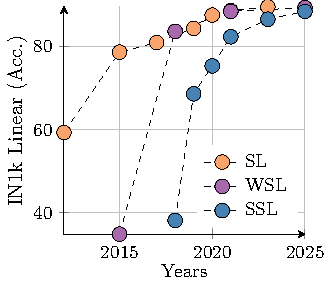
\includegraphics{figures/tikz/intro_evolution_in_time.pdf}
        

        \vspace{1.1em}
        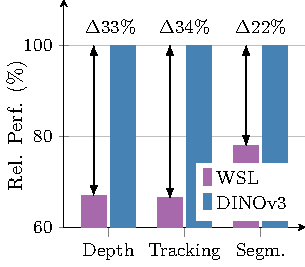
\includegraphics{figures/tikz/intro_comparison_us_bestintown.pdf} 

        \vspace{-0.2em}
    \end{minipage}%
    \hfill
    \begin{minipage}[b]{0.6\textwidth}
        \hfill
        \begin{tikzpicture}[every node/.style={inner sep=0,outer sep=0}, node distance=0.02\textwidth and 0.02\textwidth]
          \node (img1) {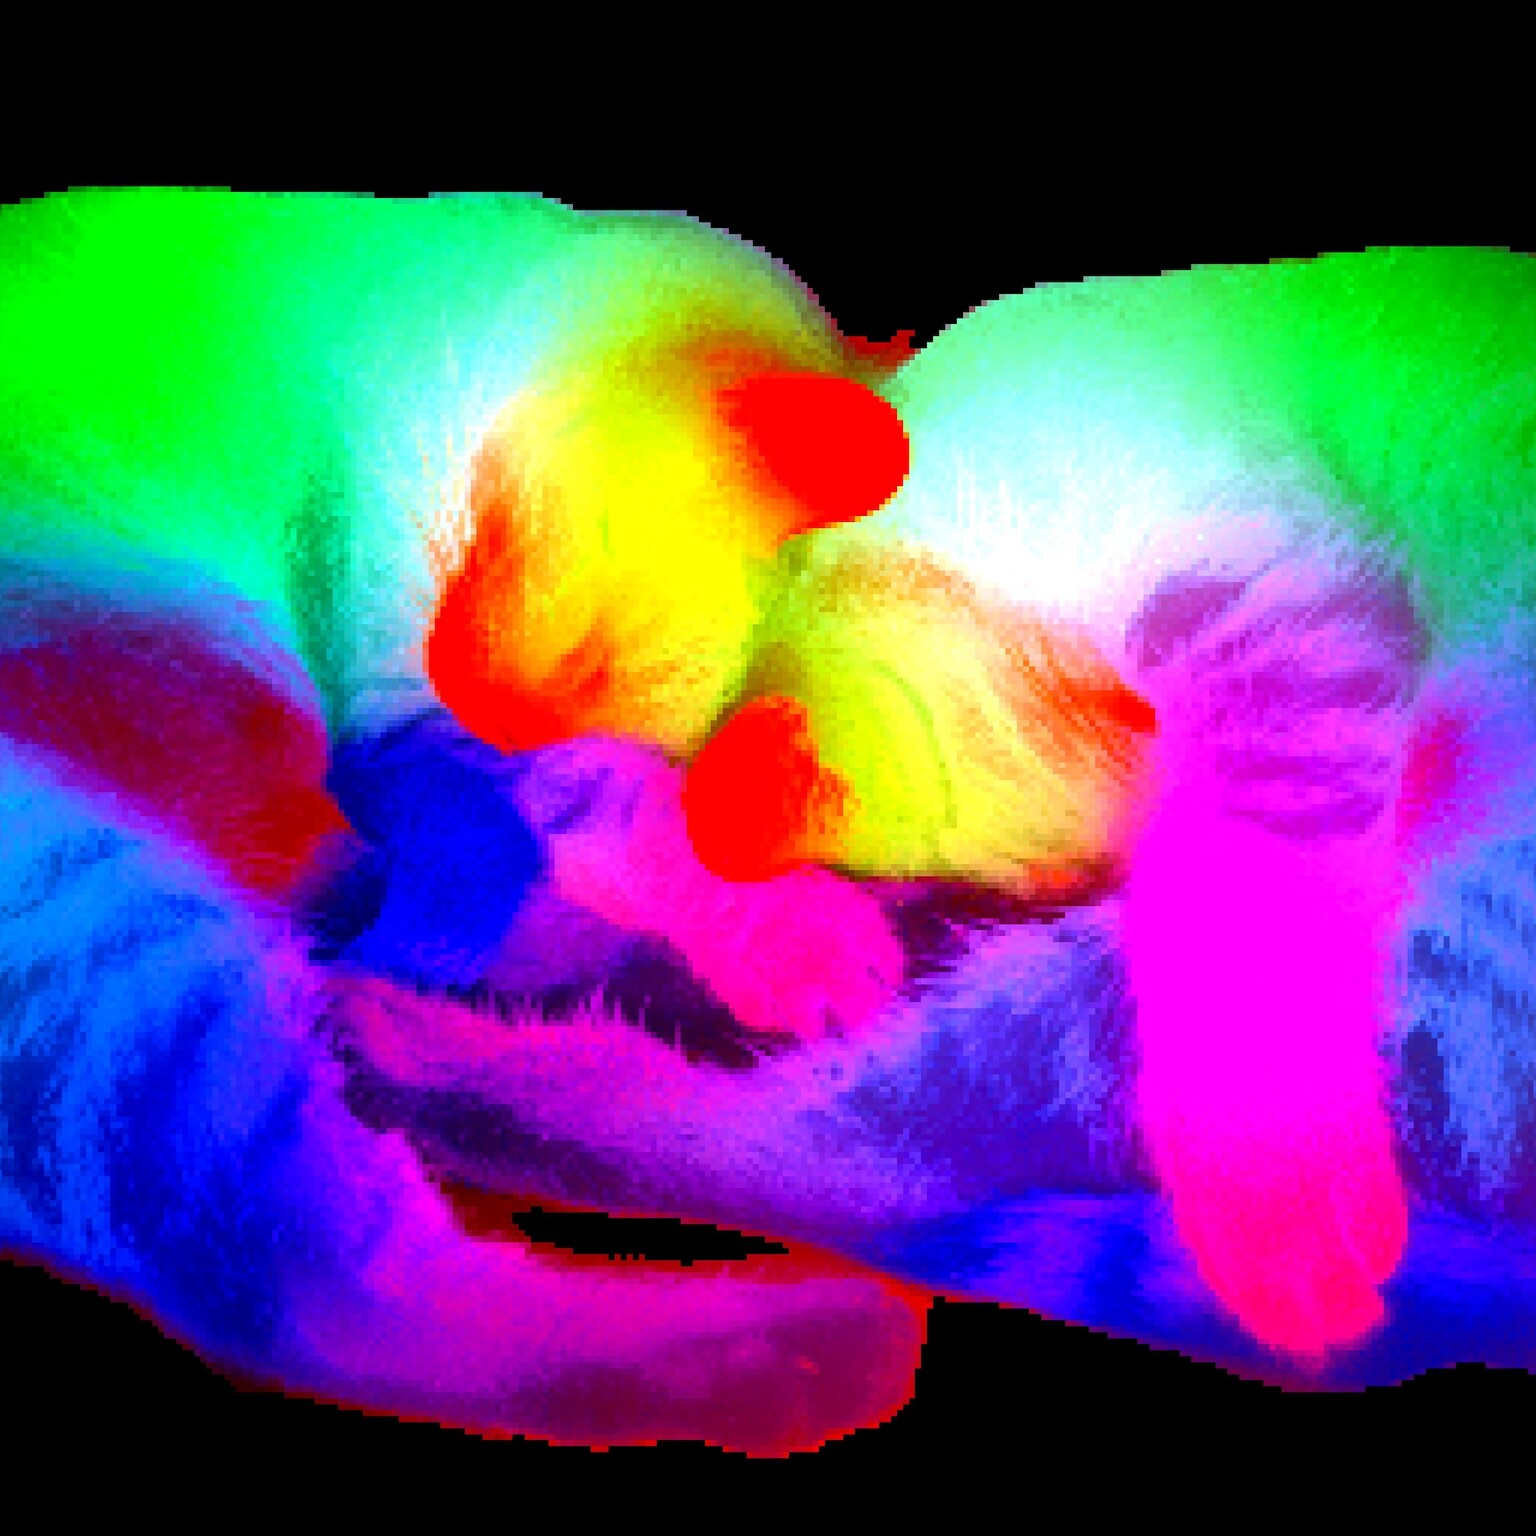
\includegraphics[width=0.49\textwidth]{figures/introduction/new_cat_pca_1.lr.jpg}};
          \node[right=of img1] (img2) {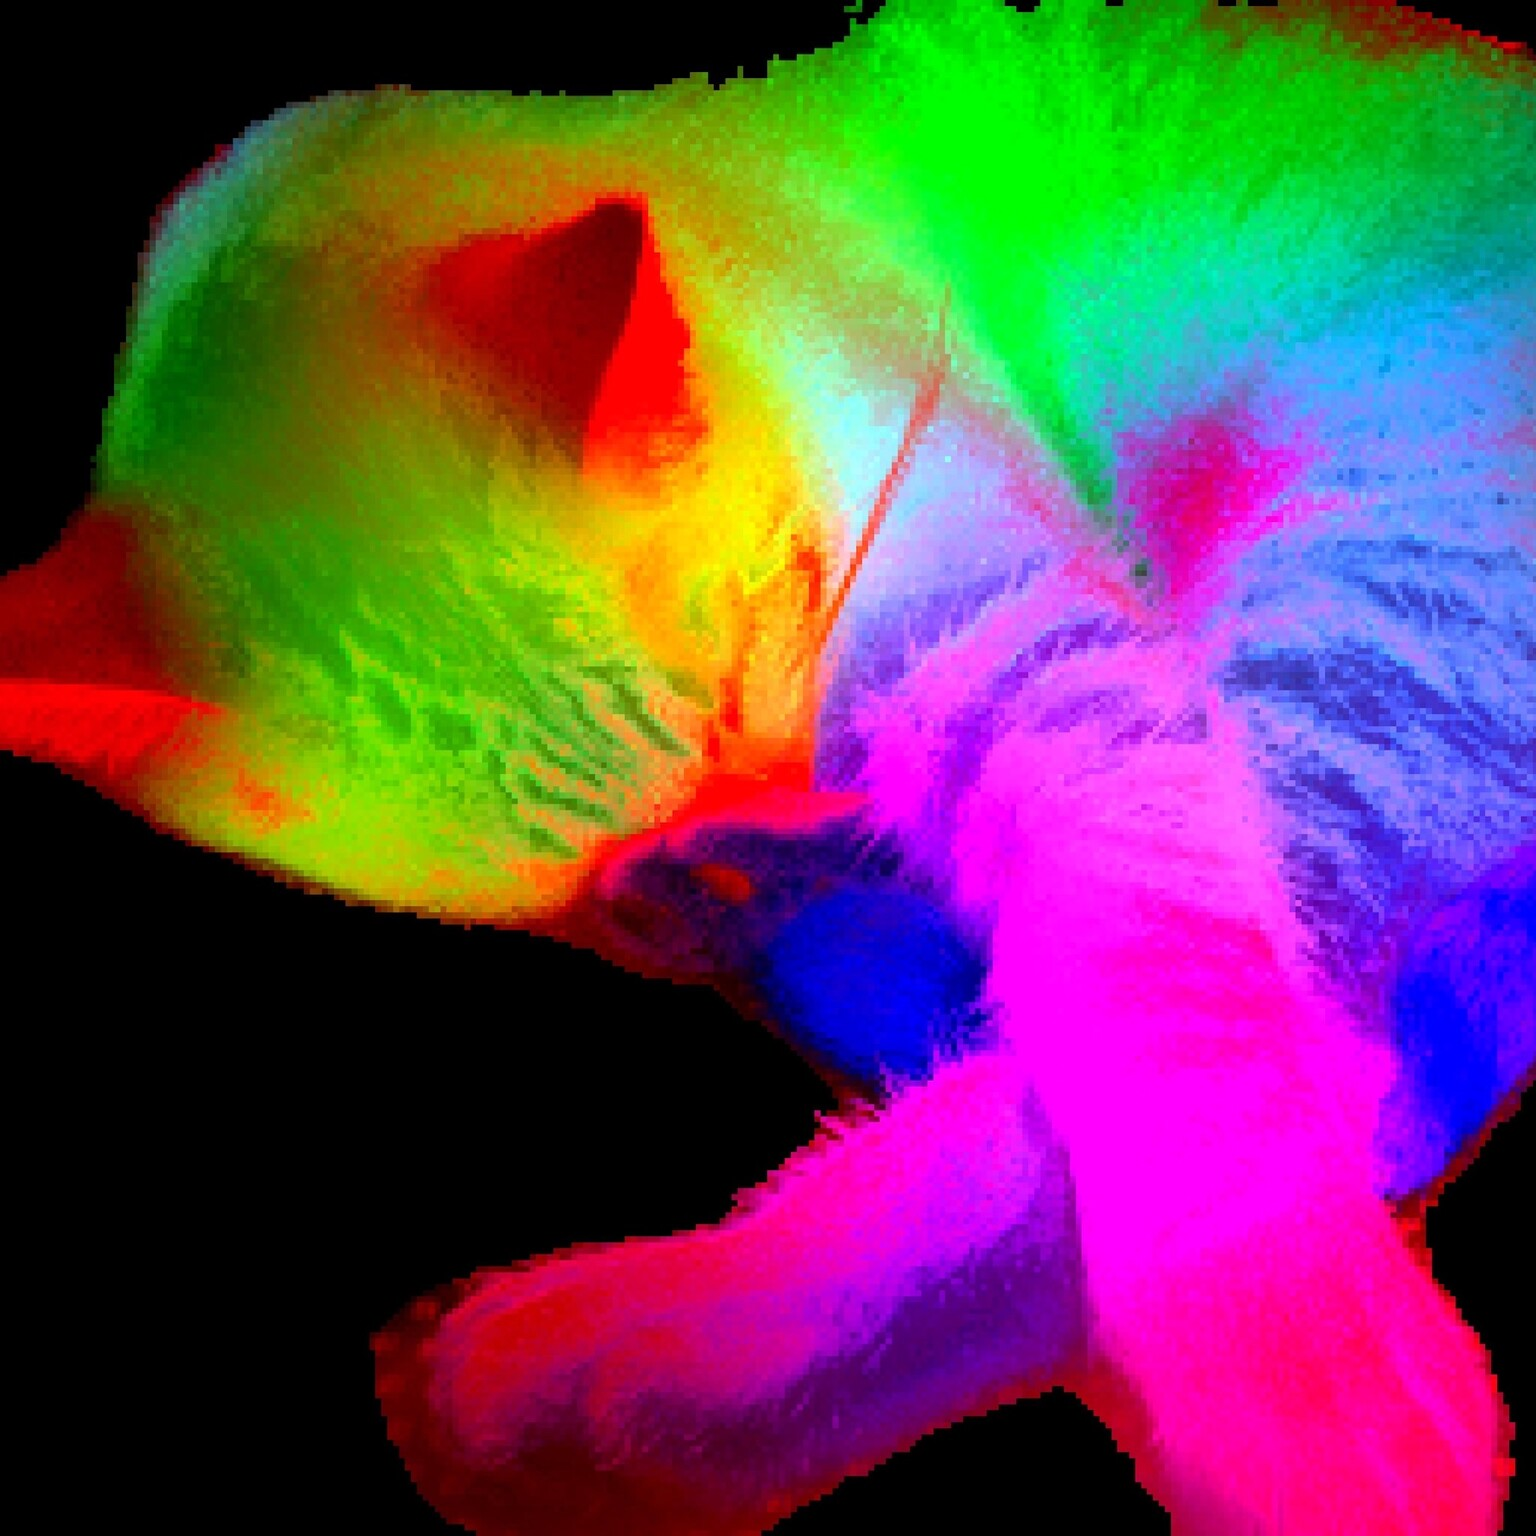
\includegraphics[width=0.49\textwidth]{figures/introduction/new_cat_pca_2.lr.jpg}};
          \node[below=of img1] (img3) {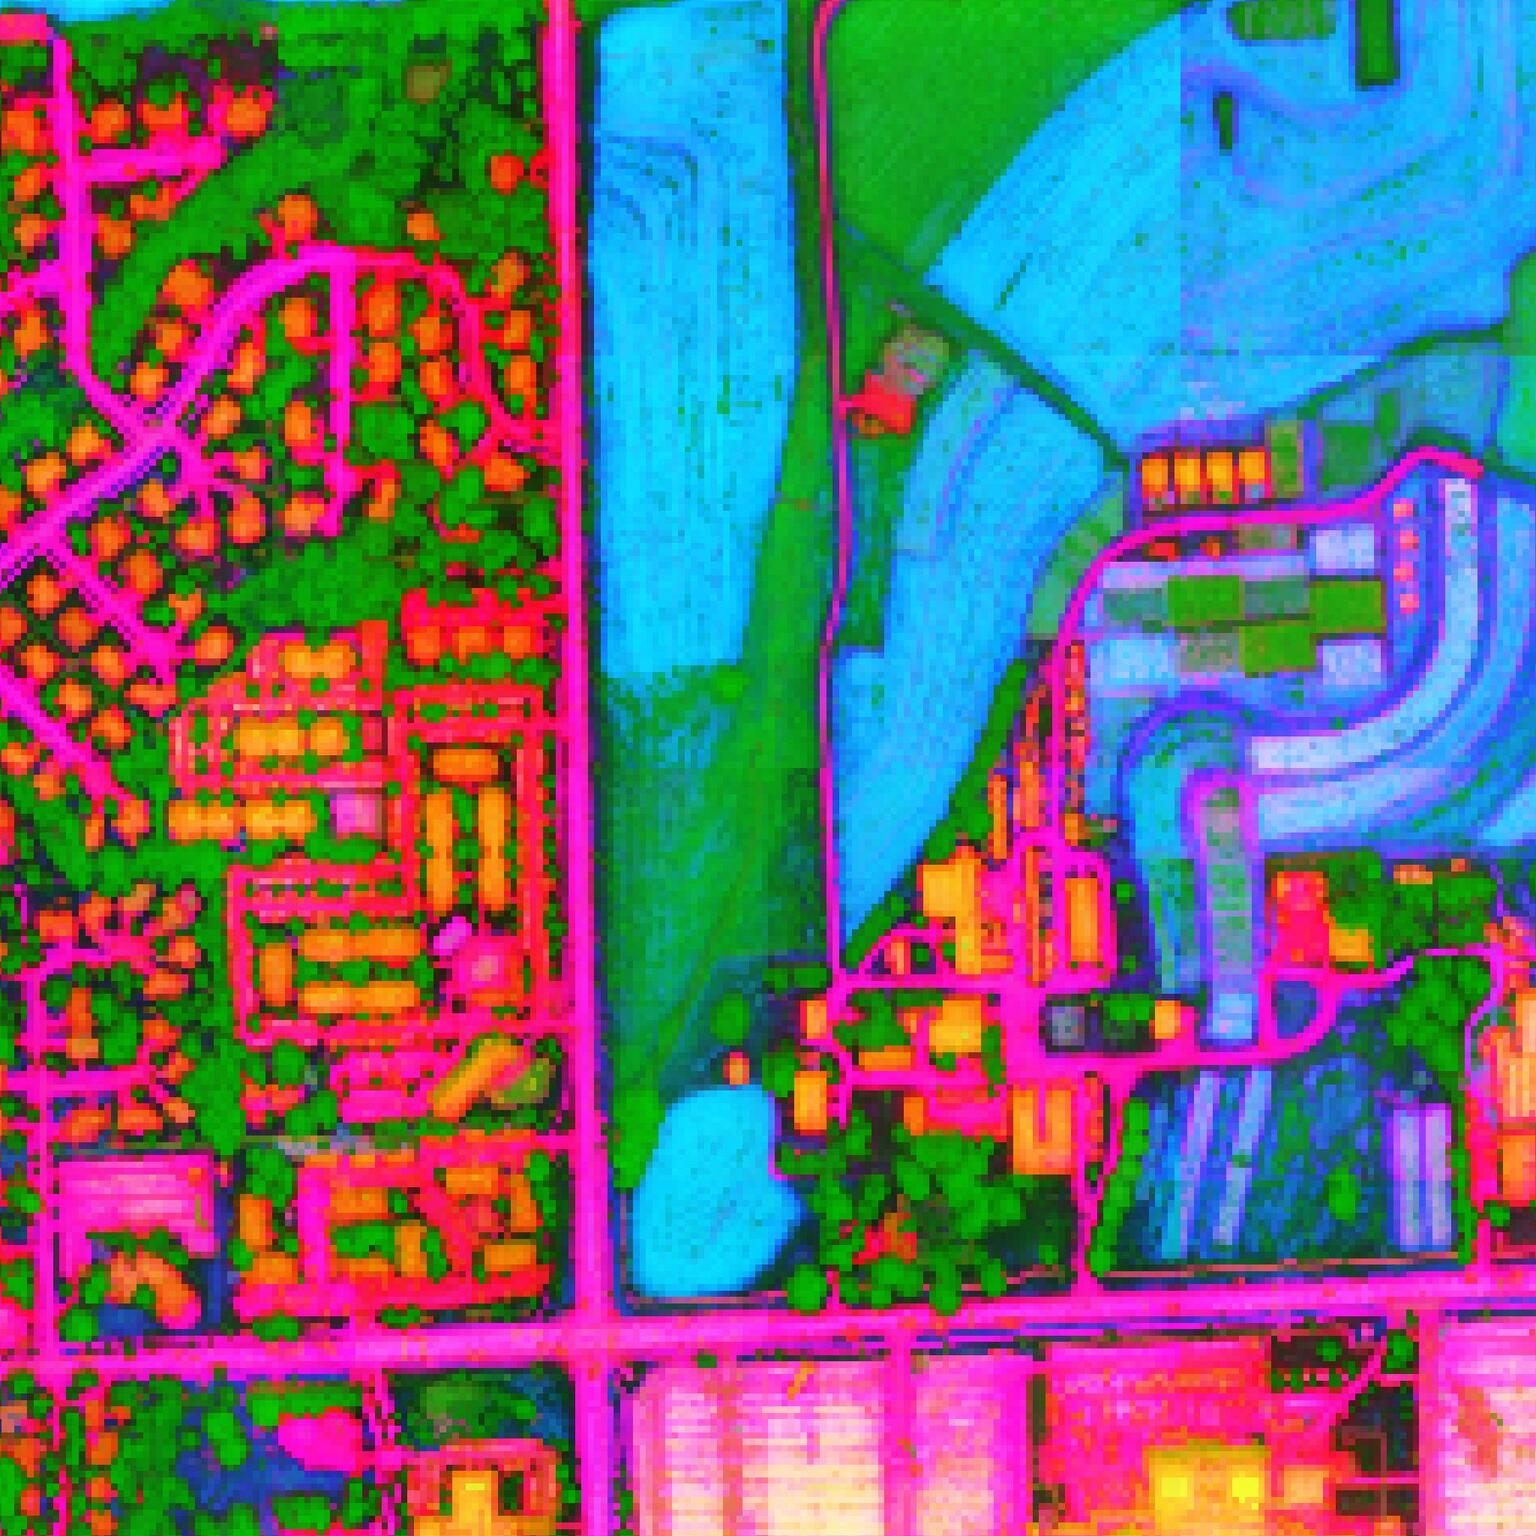
\includegraphics[width=0.49\textwidth]{figures/introduction/satellite1.lr.jpg}};
          \node[right=of img3] (img4) {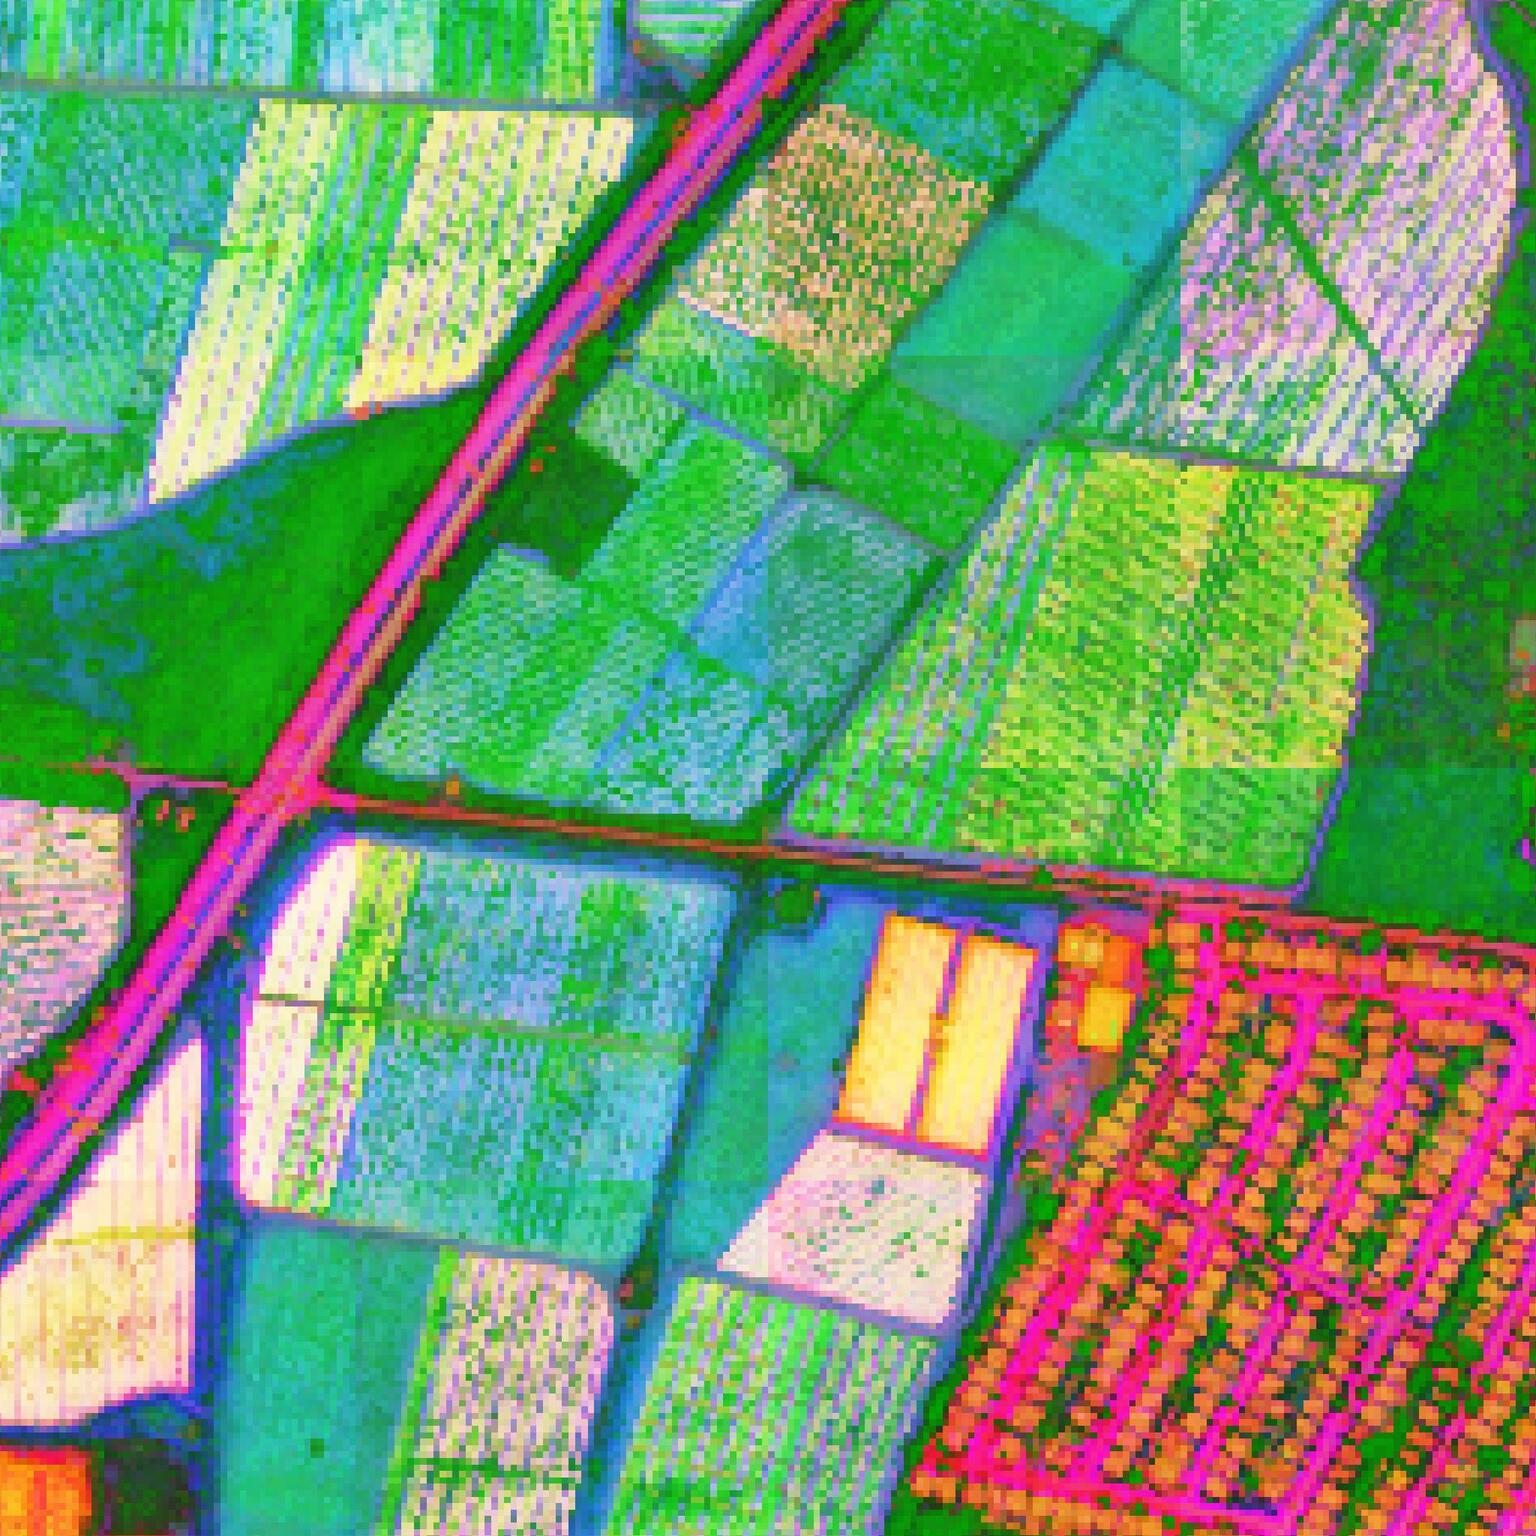
\includegraphics[width=0.49\textwidth]{figures/introduction/satellite2.lr.jpg}};
          \node[font=\bfseries,overlay] at ([xshift=-0.636\textwidth,yshift=-0.75\baselineskip]img1.north west) {(a)};
          \node[font=\bfseries,overlay,text=white] at ([xshift=0.35cm,yshift=-0.75\baselineskip]img1.north west) {(c)};
          \node[font=\bfseries,overlay] at ([xshift=-0.636\textwidth,yshift=-0.75\baselineskip]img3.north west) {(b)};
          \node[font=\bfseries,overlay,text=white] at ([xshift=0.35cm,yshift=-0.75\baselineskip]img3.north west) {(d)};
        \end{tikzpicture}
        
    \end{minipage}
    \caption{(a) Evolution of linear probing results on ImageNet1k (IN1k) over the years, comparing fully- (SL), weakly- (WSL) and self-supervised learning (SSL) methods. 
    Despite coming into the picture later, SSL has quickly progressed and now reached the Imagenet accuracy plateau of recent years. 
    On the other hand, we demonstrate that SSL offers the unique promise of high-quality dense features.
    With DINOv3, we markedly improve over weakly-supervised models on dense tasks, as shown by the relative performance of the best-in-class WSL models to DINOv3 (b).
    We also produce PCA maps of features obtained from high resolution images with DINOv3 trained on natural (c) and aerial images (d).}
    \label{fig:pcas}
\end{figure}

In practice, the promise of SSL, namely producing arbitrarily large and powerful models by leveraging large amounts of unconstrained data, remains challenging at scale. 
While model instabilities and collapse are mitigated by the heuristics proposed by \citet{oquab2024dinov2}, more problems emerge from scaling further. 
First, it is unclear how to collect useful data from unlabeled collections. 
Second, in usual training practice, employing cosine schedules implies knowing the optimization horizon a priori, which is difficult when training on large image corpora. 
Third, the performance of the features gradually decreases after early training, confirmed by visual inspection of the patch similarity maps. 
This phenomenon appears in longer training runs with models above ViT-Large size (300M parameters), reducing the usefulness of scaling DINOv2.

Addressing the problems above leads to this work, \emph{DINOv3}, which advances SSL training at scale.  
We demonstrate that a \emph{single frozen SSL backbone} can serve as a universal visual encoder that achieves state-of-the-art performance on challenging downstream tasks, outperforming supervised and metadata-reliant pre-training strategies. 
Our research is guided by the following objectives: 
(1) training a foundational model versatile across tasks and domains, 
(2) improving the shortcomings of existing SSL models on dense features, 
(3) disseminating a family of models that can be used off-the-shelf.  
We discuss the three aims in the following.

\begin{figure}[t]
    \begin{subfigure}[b]{0.35\textwidth}
        \centering
        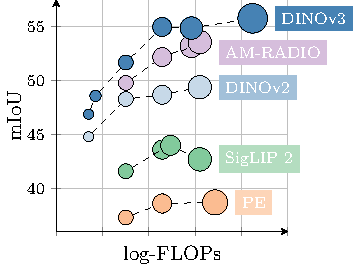
\includegraphics{figures/tikz/intro_family_models_ade20k.pdf}

        \vspace{-15pt}
        \caption{Semantic segmentation (ADE20k)}
   \end{subfigure}%
   \hfill%
    \begin{subfigure}[b]{0.30\textwidth}
        \centering
        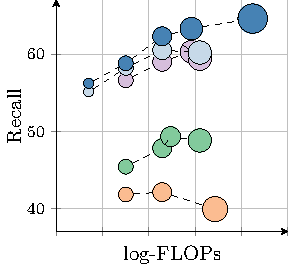
\includegraphics{figures/tikz/intro_family_models_probe3d.pdf}

        \vspace{-15pt}
        \caption{3D keypoint matching (NAVI)}
   \end{subfigure}%
   \hfill%
    \begin{subfigure}[b]{0.30\textwidth}
        \centering
        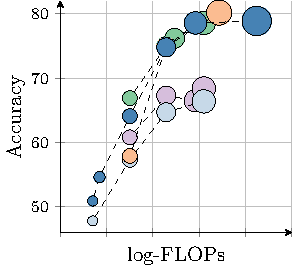
\includegraphics{figures/tikz/intro_family_models_objectnet.pdf}

        \vspace{-15pt}
        \caption{OOD classif. (ObjectNet)}
   \end{subfigure}
   \caption{Performance of the DINOv3 family of models, compared to other families of self- or weakly-supervised models, on different benchmarks. DINOv3 significantly surpasses others on dense benchmarks, including models that leverage mask annotation priors such as AM-RADIO~\citep{heinrich2025radiov25}.}
   \label{fig:intro:family}
\end{figure}

\paragraph{Strong \& Versatile Foundational Models}  
DINOv3 aims to offer a high level of versatility along two axes, which is enabled by the scaling of the model size and training data. 
First, a key desirable property for SSL models is to achieve excellent performance while being kept frozen, ideally reaching similar state-of-the-art results as specialized models. 
In that case, a single forward pass can deliver cutting-edge results across multiple tasks, leading to substantial computational savings---an essential advantage for practical applications, particularly on edge devices. 
We show the wide breadth of tasks that DINOv3 can successfully be applied to in \cref{sec:results}.
Second, a scalable SSL training pipeline that does not depend on metadata unlocks numerous scientific applications. 
By pre-training on a diverse set of images, whether web images or observational data, SSL models generalize across a large set of domains and tasks. 
As illustrated in \cref{fig:pcas}(d), the PCA of DINOv3 features extracted from a high-resolution aerial image clearly allows to separates roads, houses, and greenery, highlighting the model’s feature quality. 

\paragraph[Superior Feature Maps Through Gram]{Superior Feature Maps Through \Gramname}
Another key feature of DINOv3 is a significant improvement of its dense feature maps. 
The DINOv3 SSL training strategy aims at producing models excelling at high-level semantic tasks while producing excellent feature maps amenable to solving geometric tasks such as depth estimation, or 3D matching.
In particular, the models should produce dense features that can be used off-the-shelf or with little post-processing. 
The compromise between dense and global representation is especially difficult to optimize when training with vast amounts of images, since the objective of high-level understanding can conflict with the quality of the dense feature maps. 
These contradictory objectives lead to a collapse of dense features with large models and long training schedules.
Our new \gramname strategy effectively mitigates this collapse (see \cref{sec:gram}).
As a result, DINOv3 obtains significantly better dense feature maps than DINOv2, staying clean even at high resolutions (see \cref{fig:intro:dense-quality}). 

\paragraph{The DINOv3 Family of Models} 
Solving the degradation of dense feature map with \gramname unlocks the power of scaling.
As a consequence, training a much larger model with SSL leads to significant performance improvements. 
In this work, we successfully train a DINO model with 7B parameters. 
Since such a large model requires significant resources to run, we apply distillation to compress its knowledge into smaller variants. 
As a result, we present the \emph{DINOv3 family of vision models}, a comprehensive suite designed to address a wide spectrum of computer vision challenges. 
This model family aims to advance the state of the art by offering scalable solutions adaptable to diverse resource constraints and deployment scenarios.
The distillation process produces model variants at multiple scales, including Vision Transformer (ViT) Small, Base, and Large, as well as ConvNeXt-based architectures.
Notably, the efficient and widely adopted ViT-L model achieves performance close to that of the original 7B teacher across a variety of tasks. 
Overall, the DINOv3 family demonstrates strong performance on a broad range of benchmarks, matching or exceeding the accuracy of competing models on global tasks, while significantly outperforming them on dense prediction tasks, as visible in \cref{fig:intro:family}.




    
             


        
                            

            

            
                
        
                            

            

            
                
        
            


            

            
        
            


            

            
        
            



            


\begin{figure}[t]
\begin{minipage}{\linewidth}
    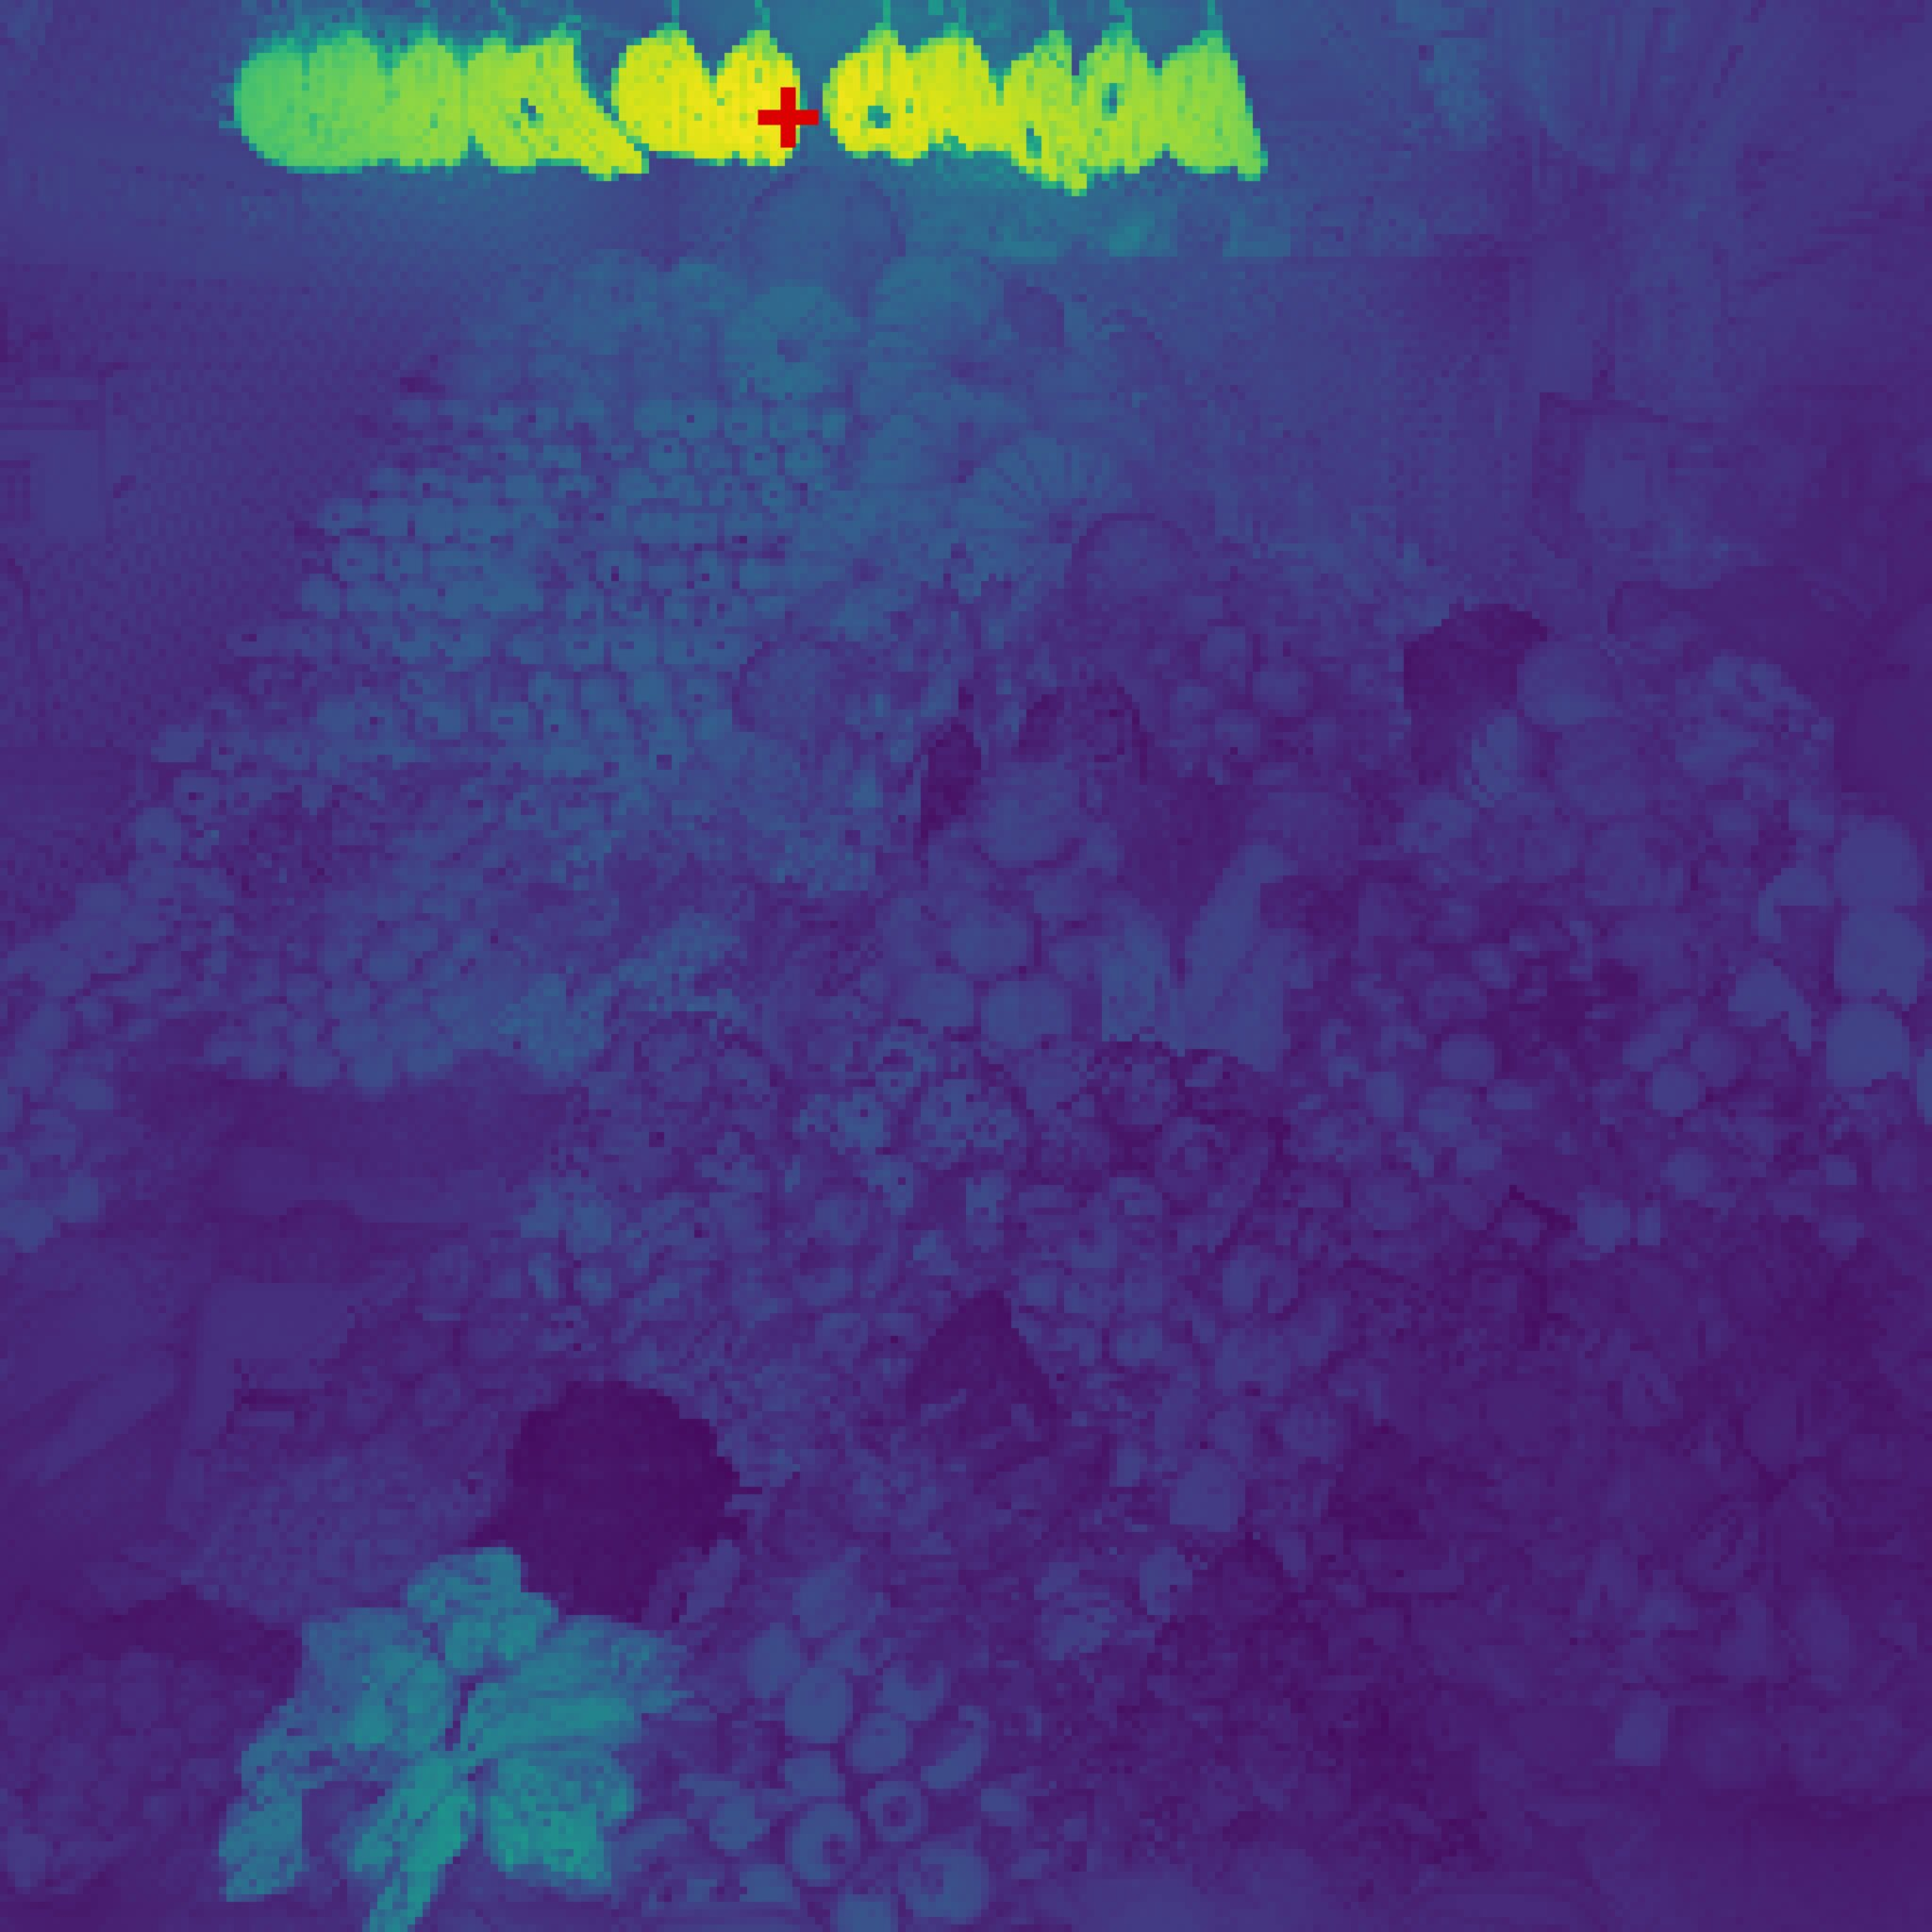
\includegraphics[height=0.248\linewidth, width=0.248\linewidth]{figures/introduction/clutter_scene/viridis_hd/cosmap_0_cross.lr.jpg}\hfill%
    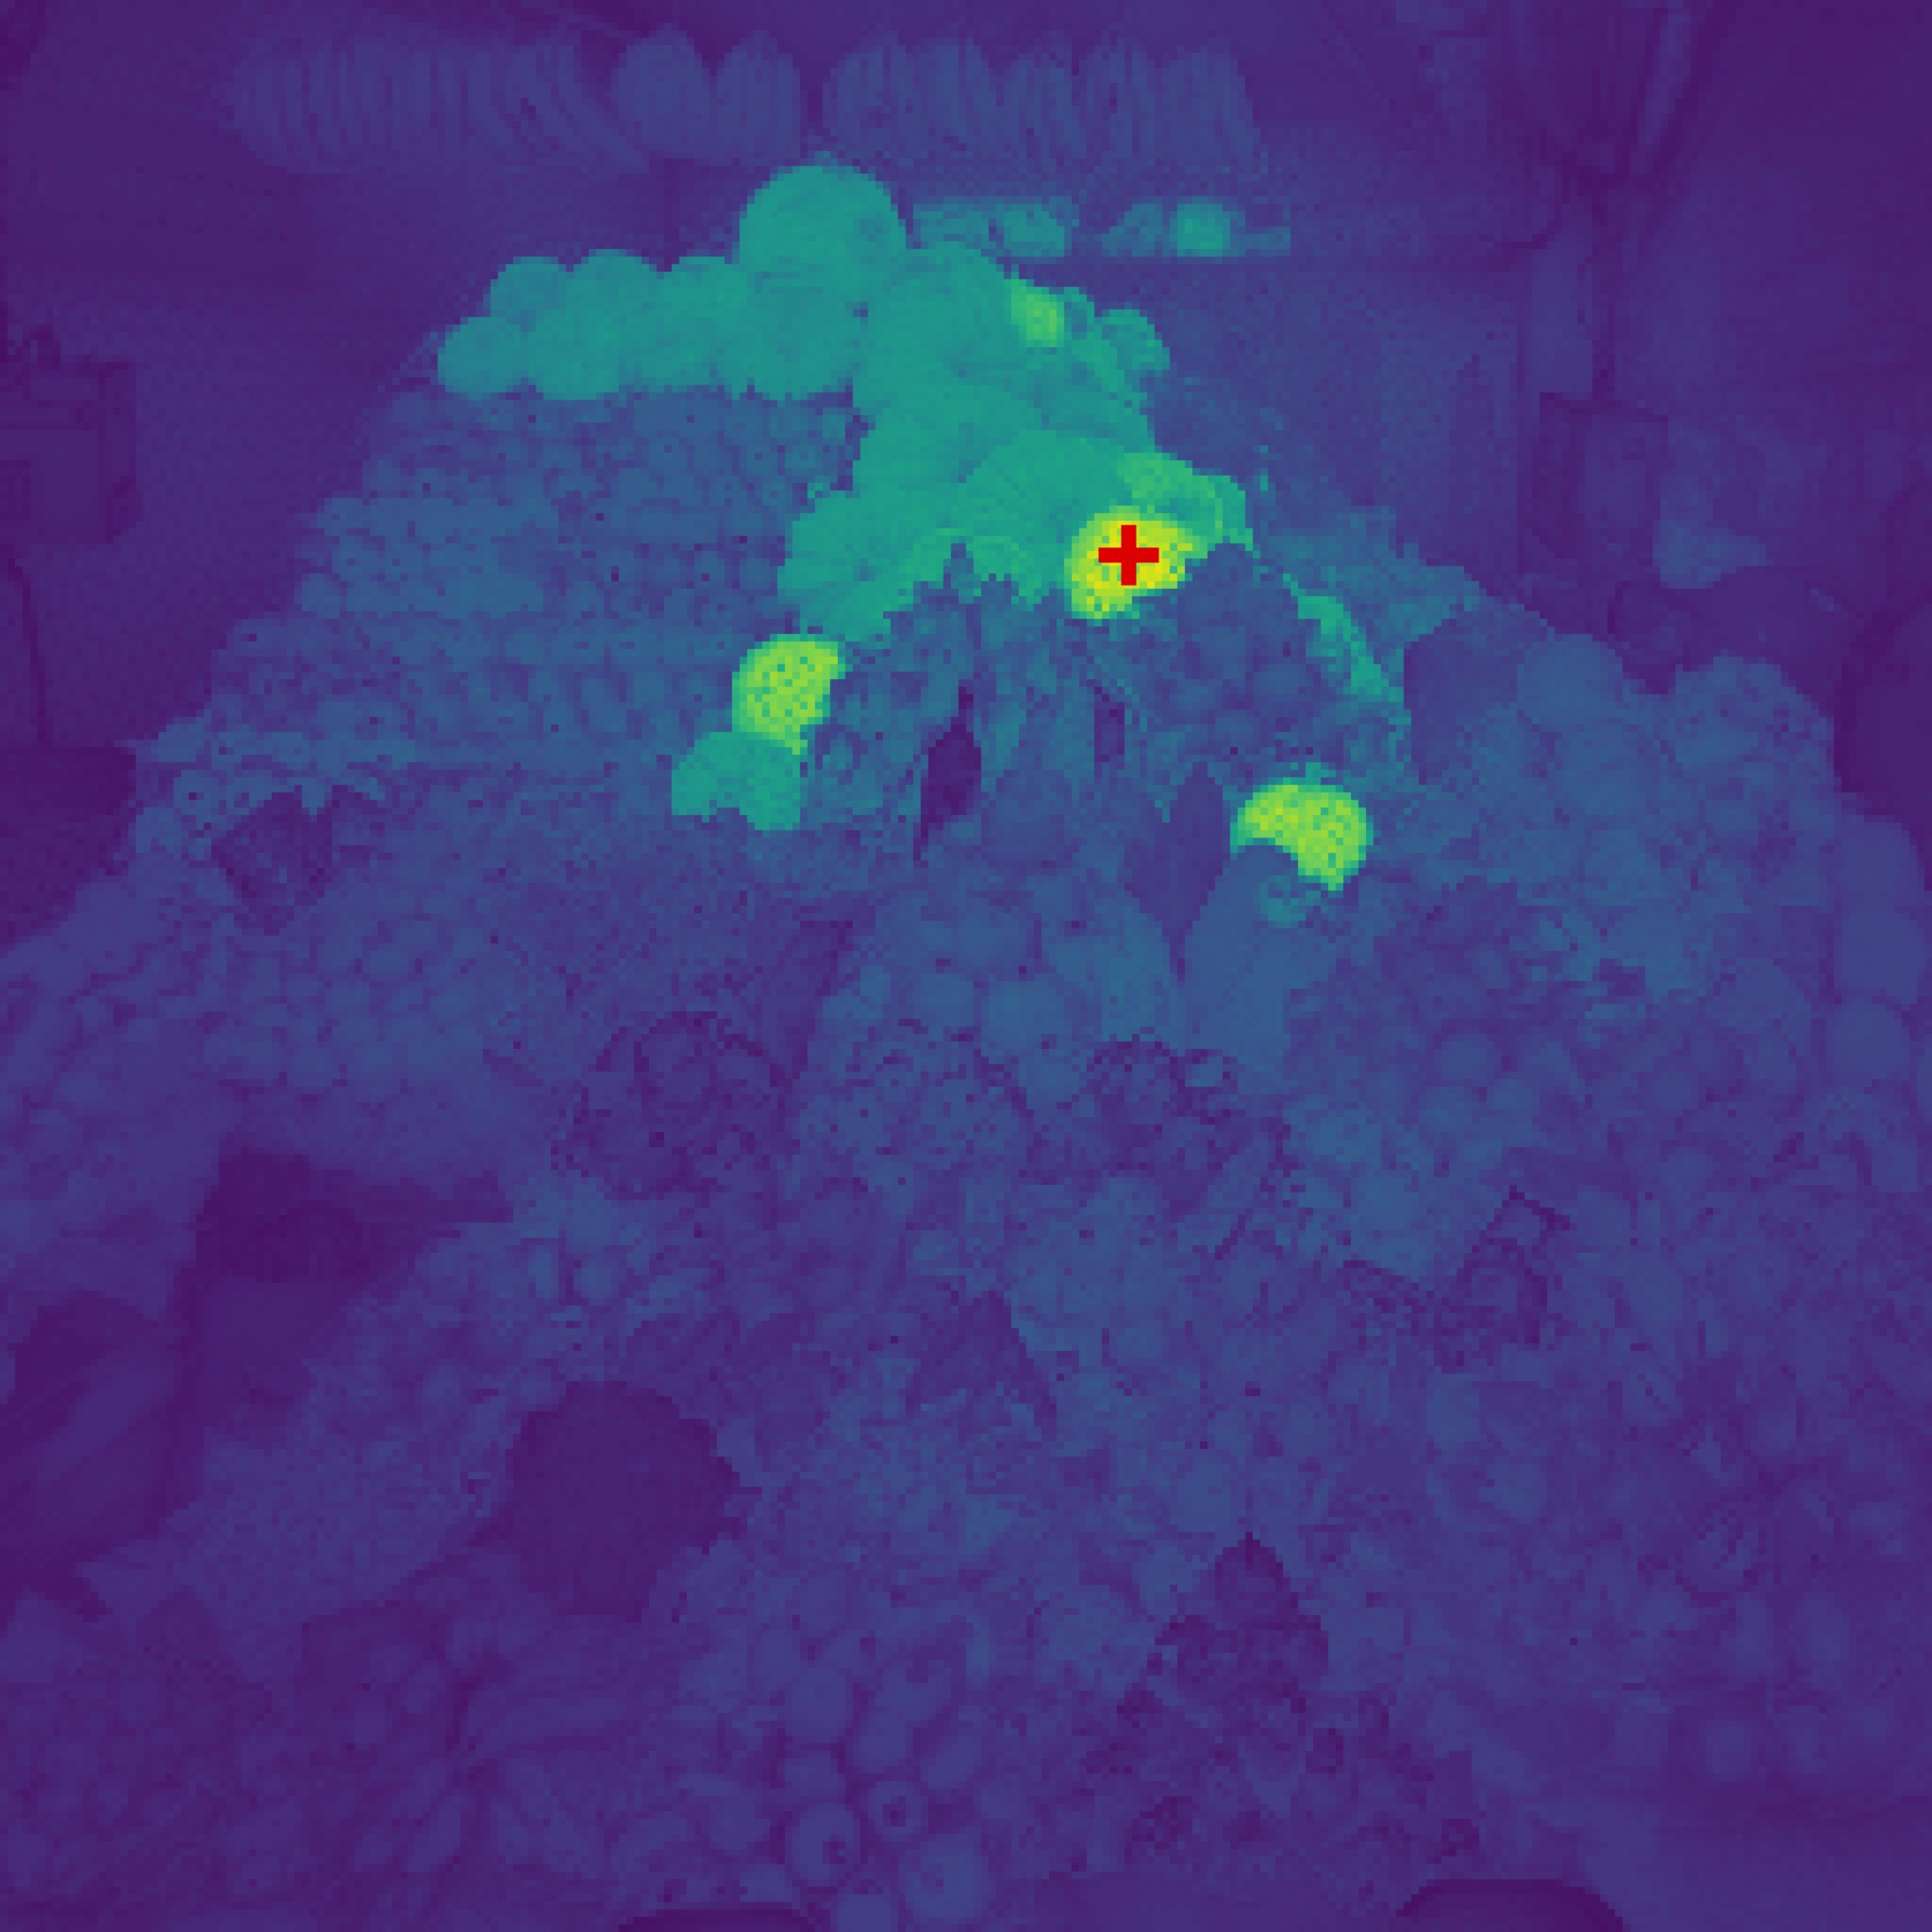
\includegraphics[height=0.248\linewidth, width=0.248\linewidth]{figures/introduction/clutter_scene/viridis_hd/cosmap_10_cross.lr.jpg}\hfill%
    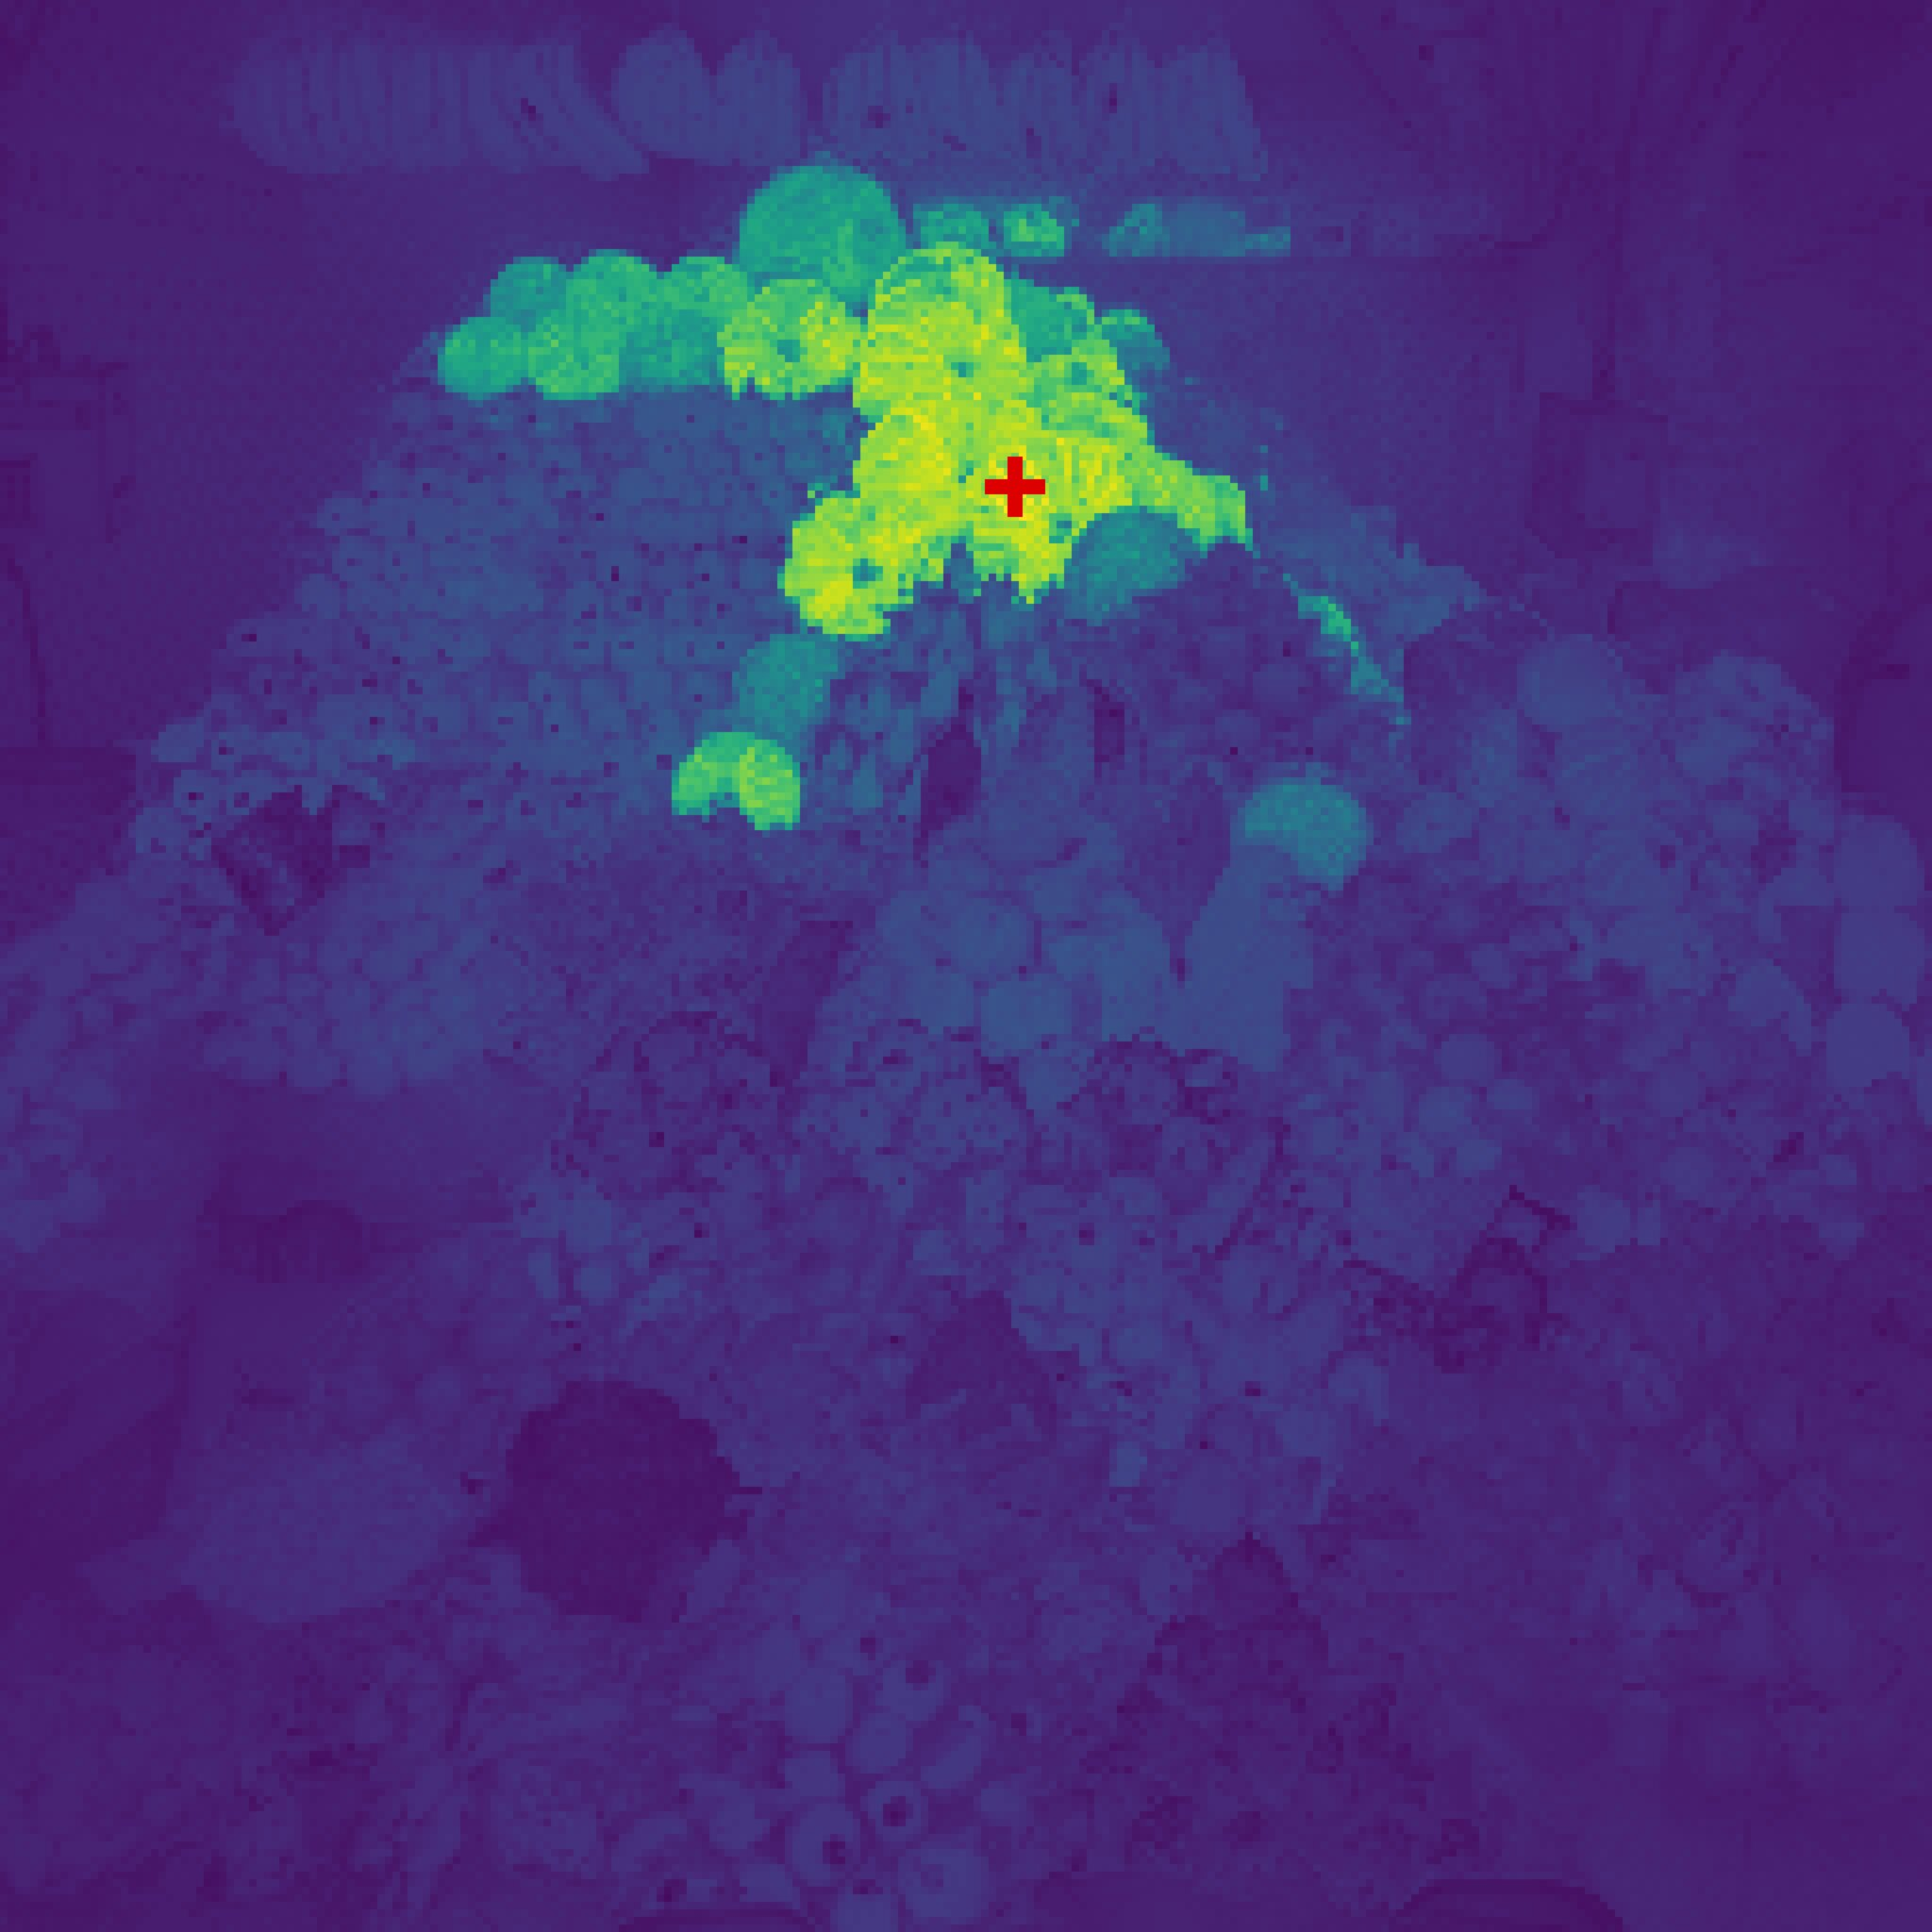
\includegraphics[height=0.248\linewidth, width=0.248\linewidth]{figures/introduction/clutter_scene/viridis_hd/cosmap_2_cross.lr.jpg}\hfill%
    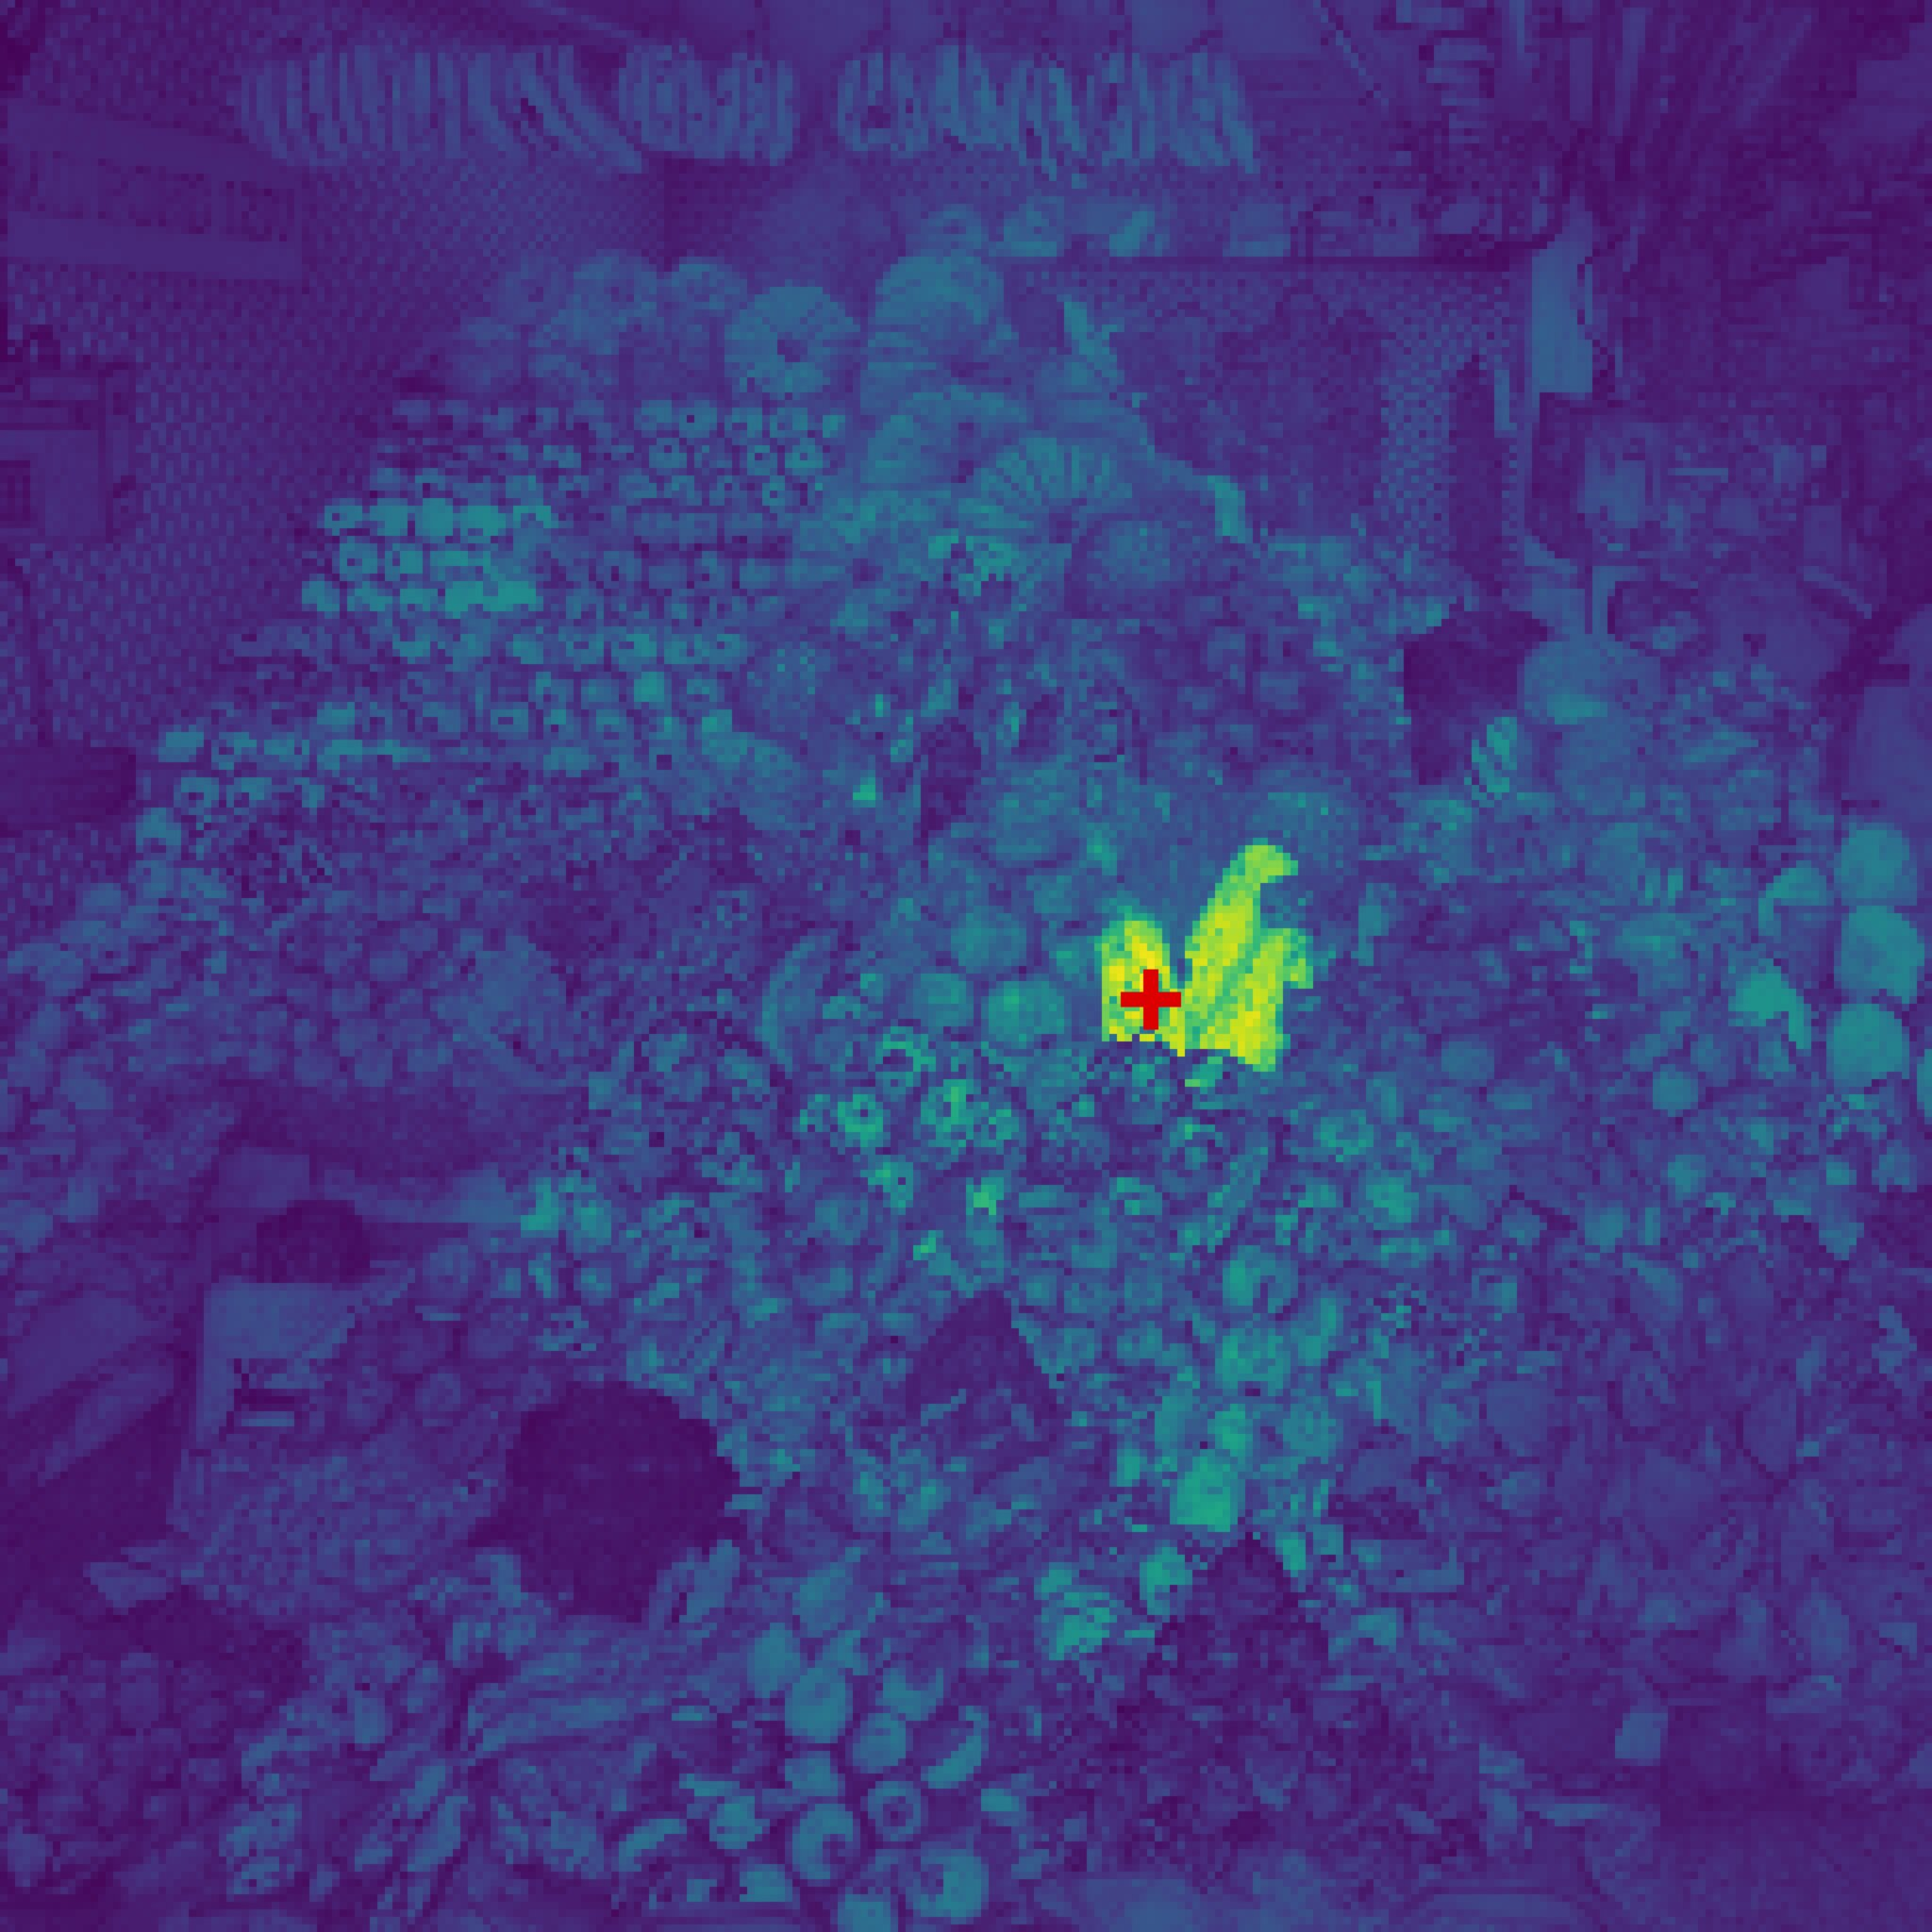
\includegraphics[height=0.248\linewidth, width=0.248\linewidth] {figures/introduction/clutter_scene/viridis_hd/cosmap_4_cross.lr.jpg}
\end{minipage}\\
\begin{minipage}{0.248\linewidth}
    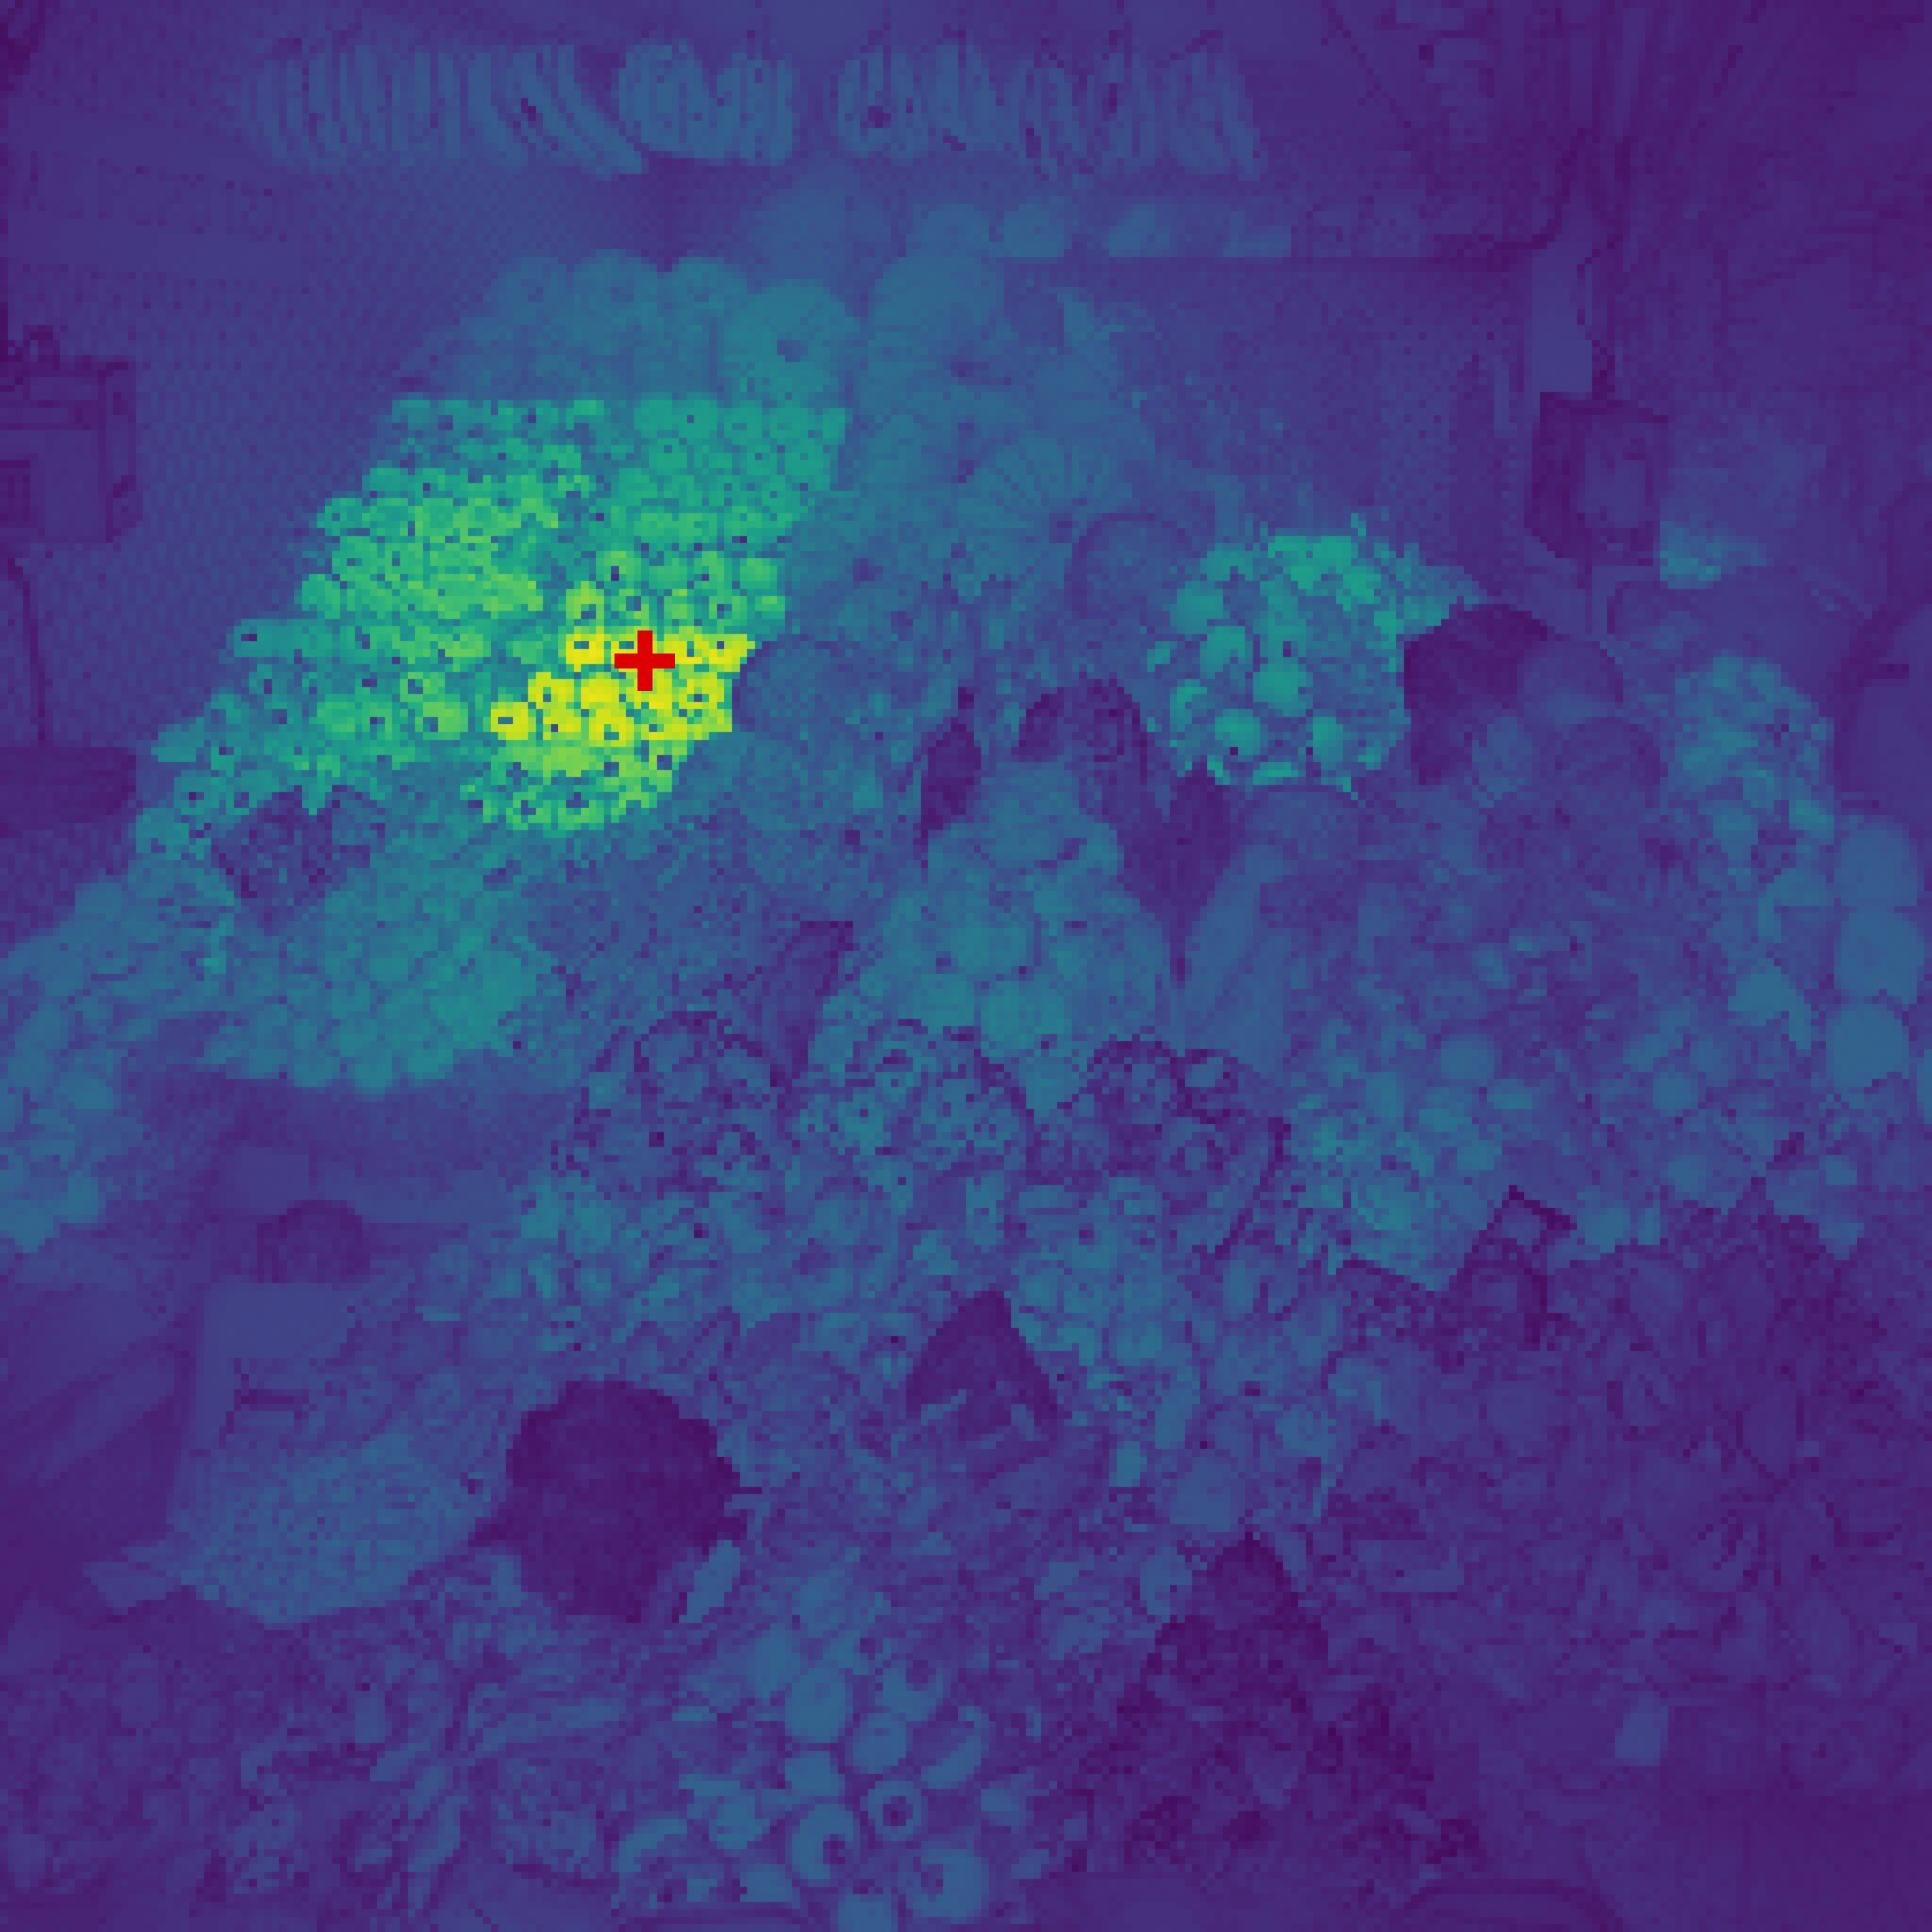
\includegraphics[height=\linewidth, width=\linewidth]{figures/introduction/clutter_scene/viridis_hd/cosmap_6_cross.lr.jpg}\\
    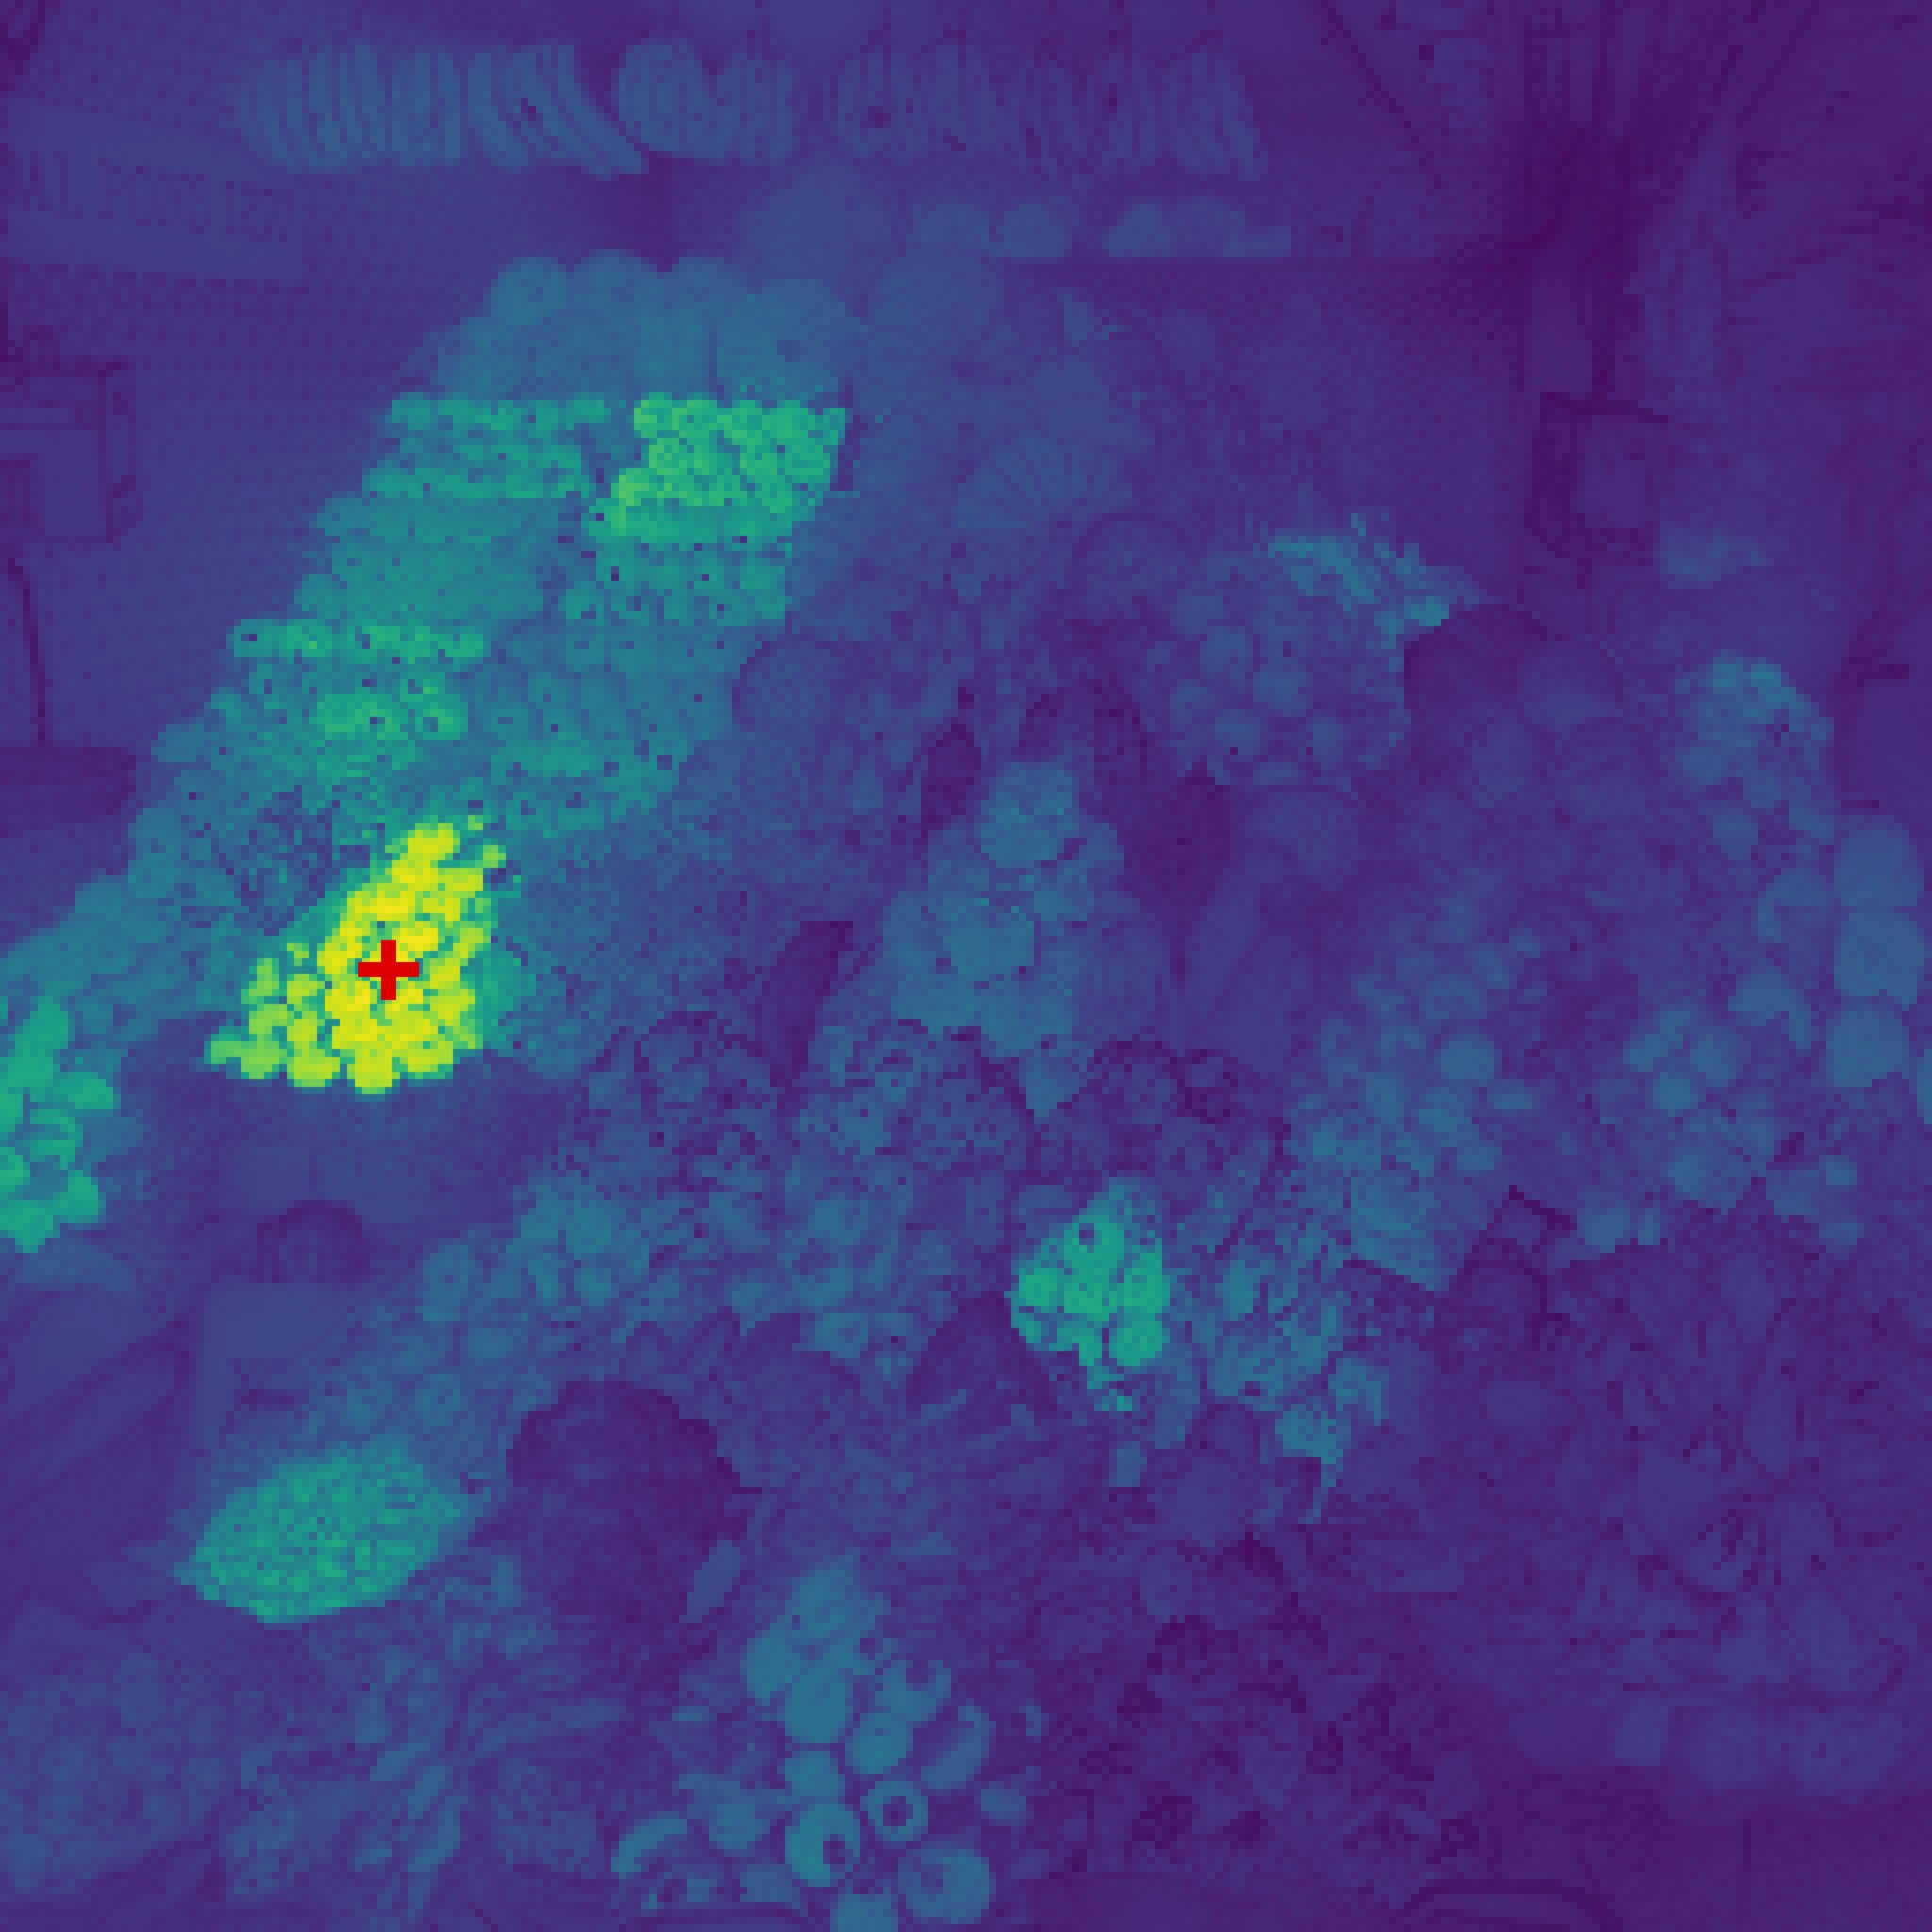
\includegraphics[height=\linewidth, width=\linewidth]{figures/introduction/clutter_scene/viridis_hd/cosmap_9_cross.lr.jpg}
\end{minipage}\hfill%
\begin{minipage}{0.499\linewidth}%
    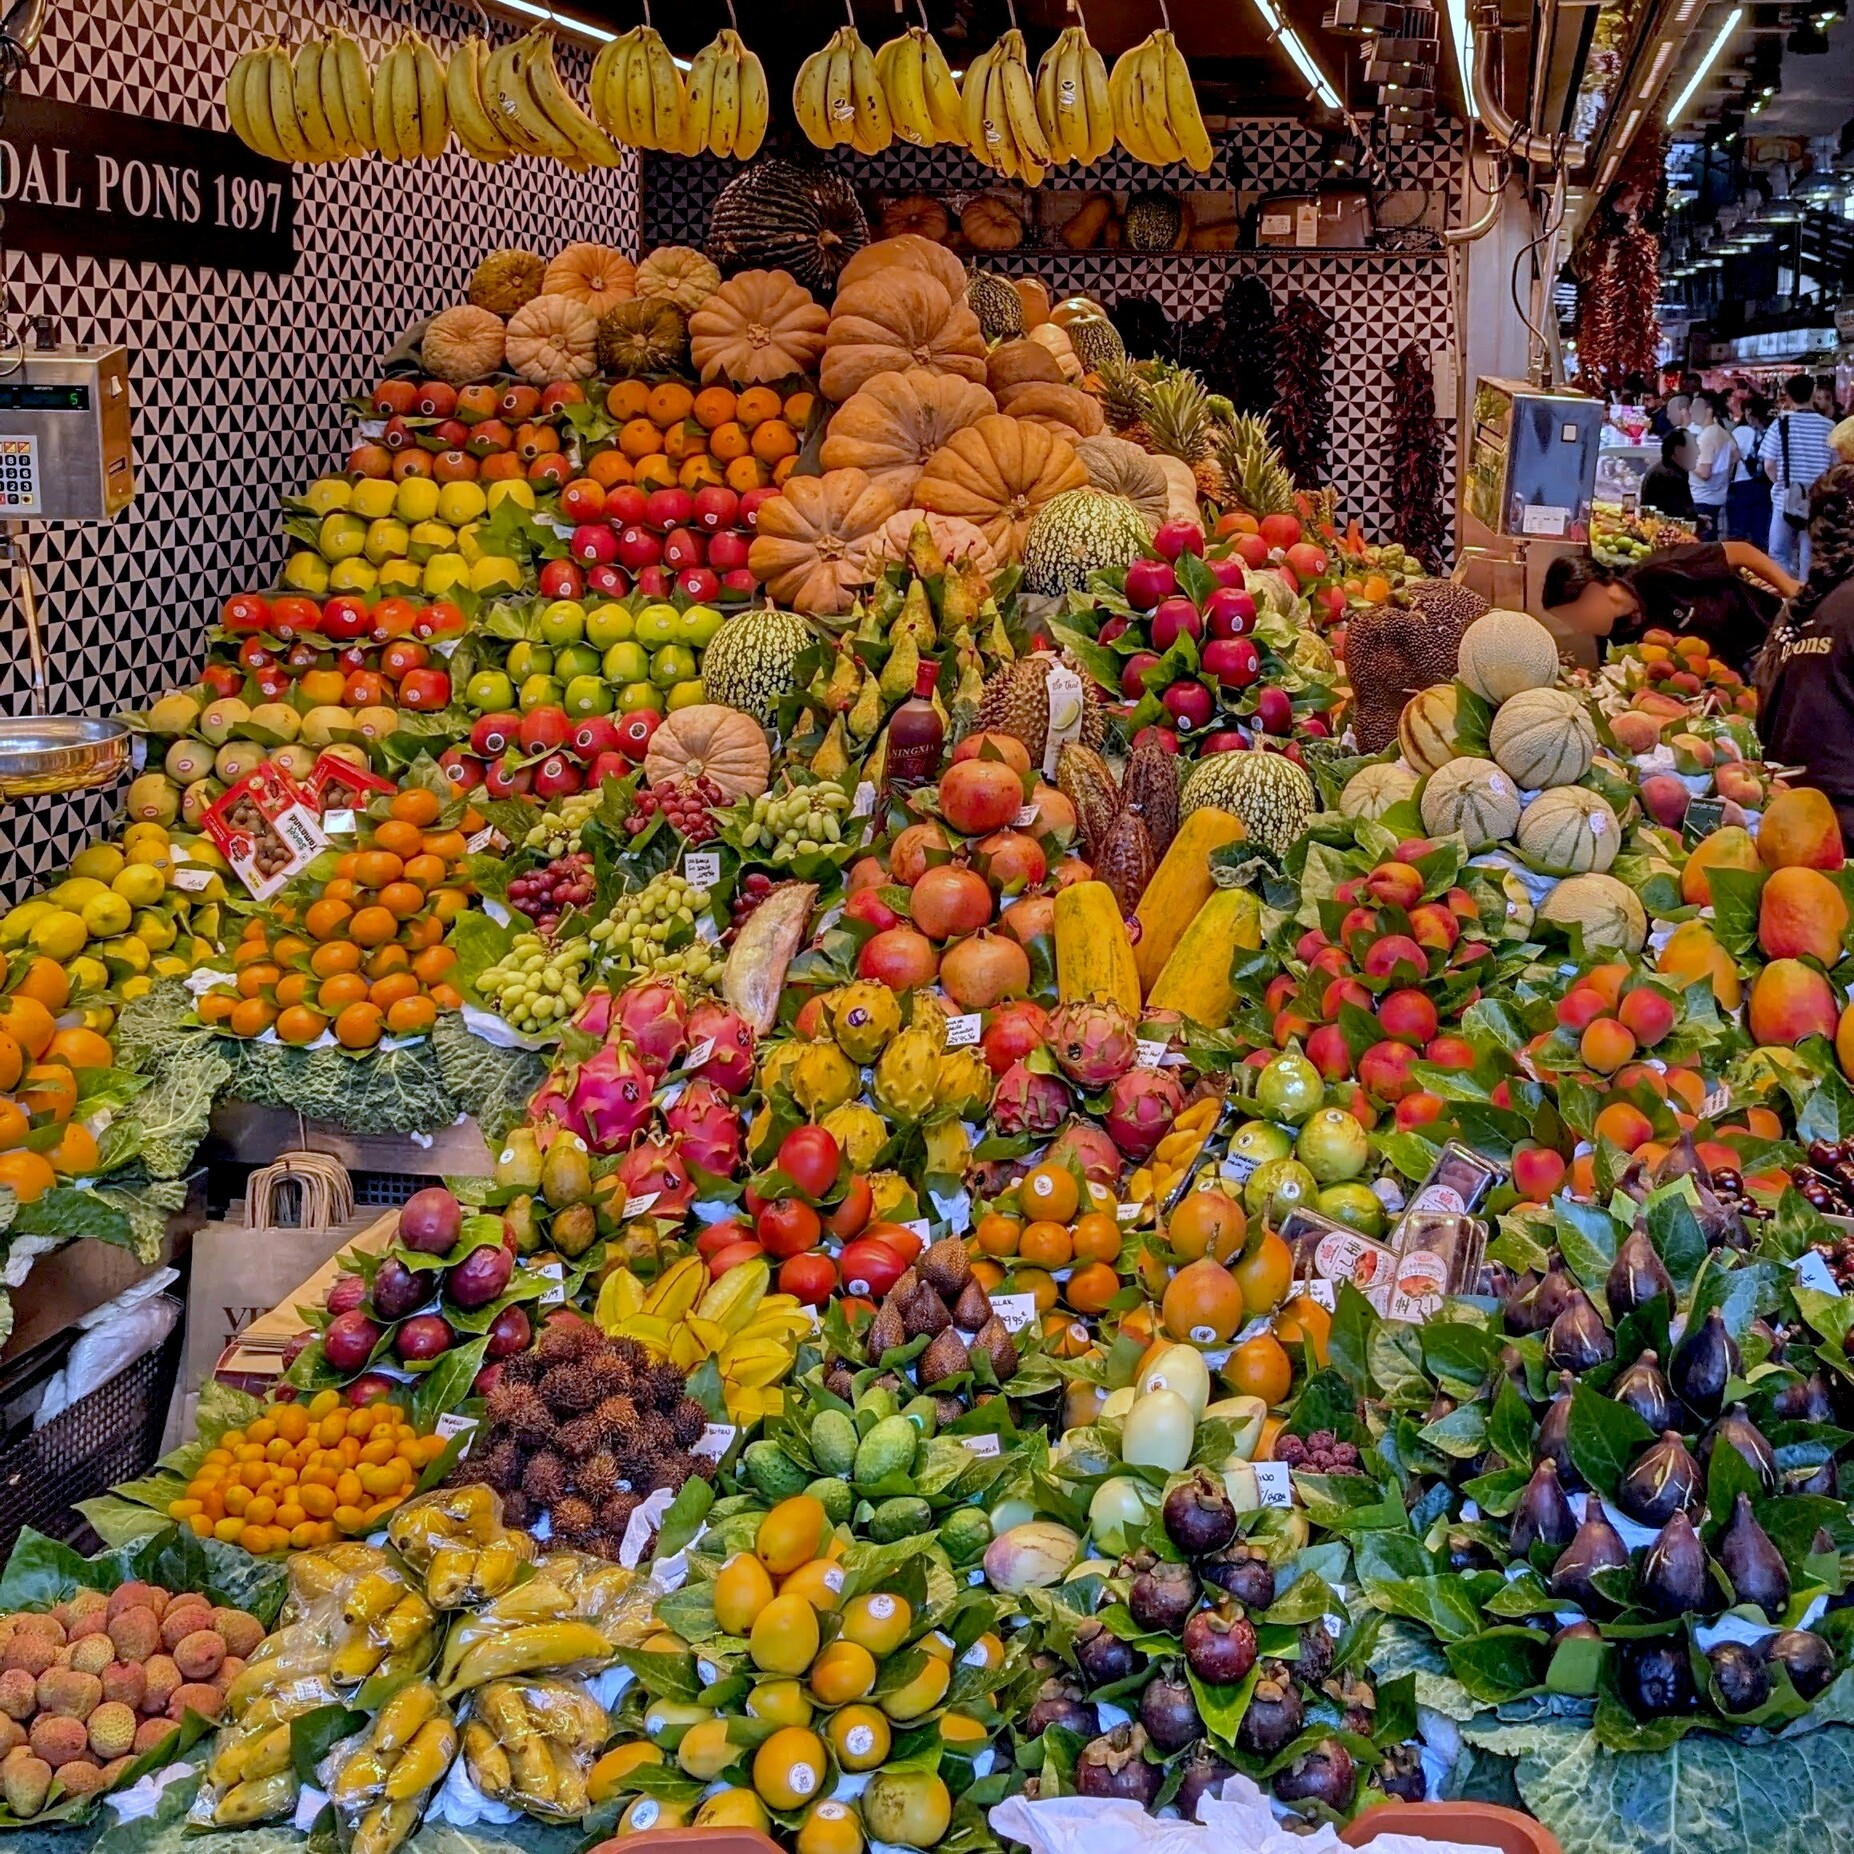
\includegraphics[height=0.998\linewidth, width=1\linewidth]{figures/introduction/clutter_scene/market_cropped_coloredit2_faceblur.lr.jpeg}%
\end{minipage}\hfill%
\begin{minipage}{0.248\linewidth}
    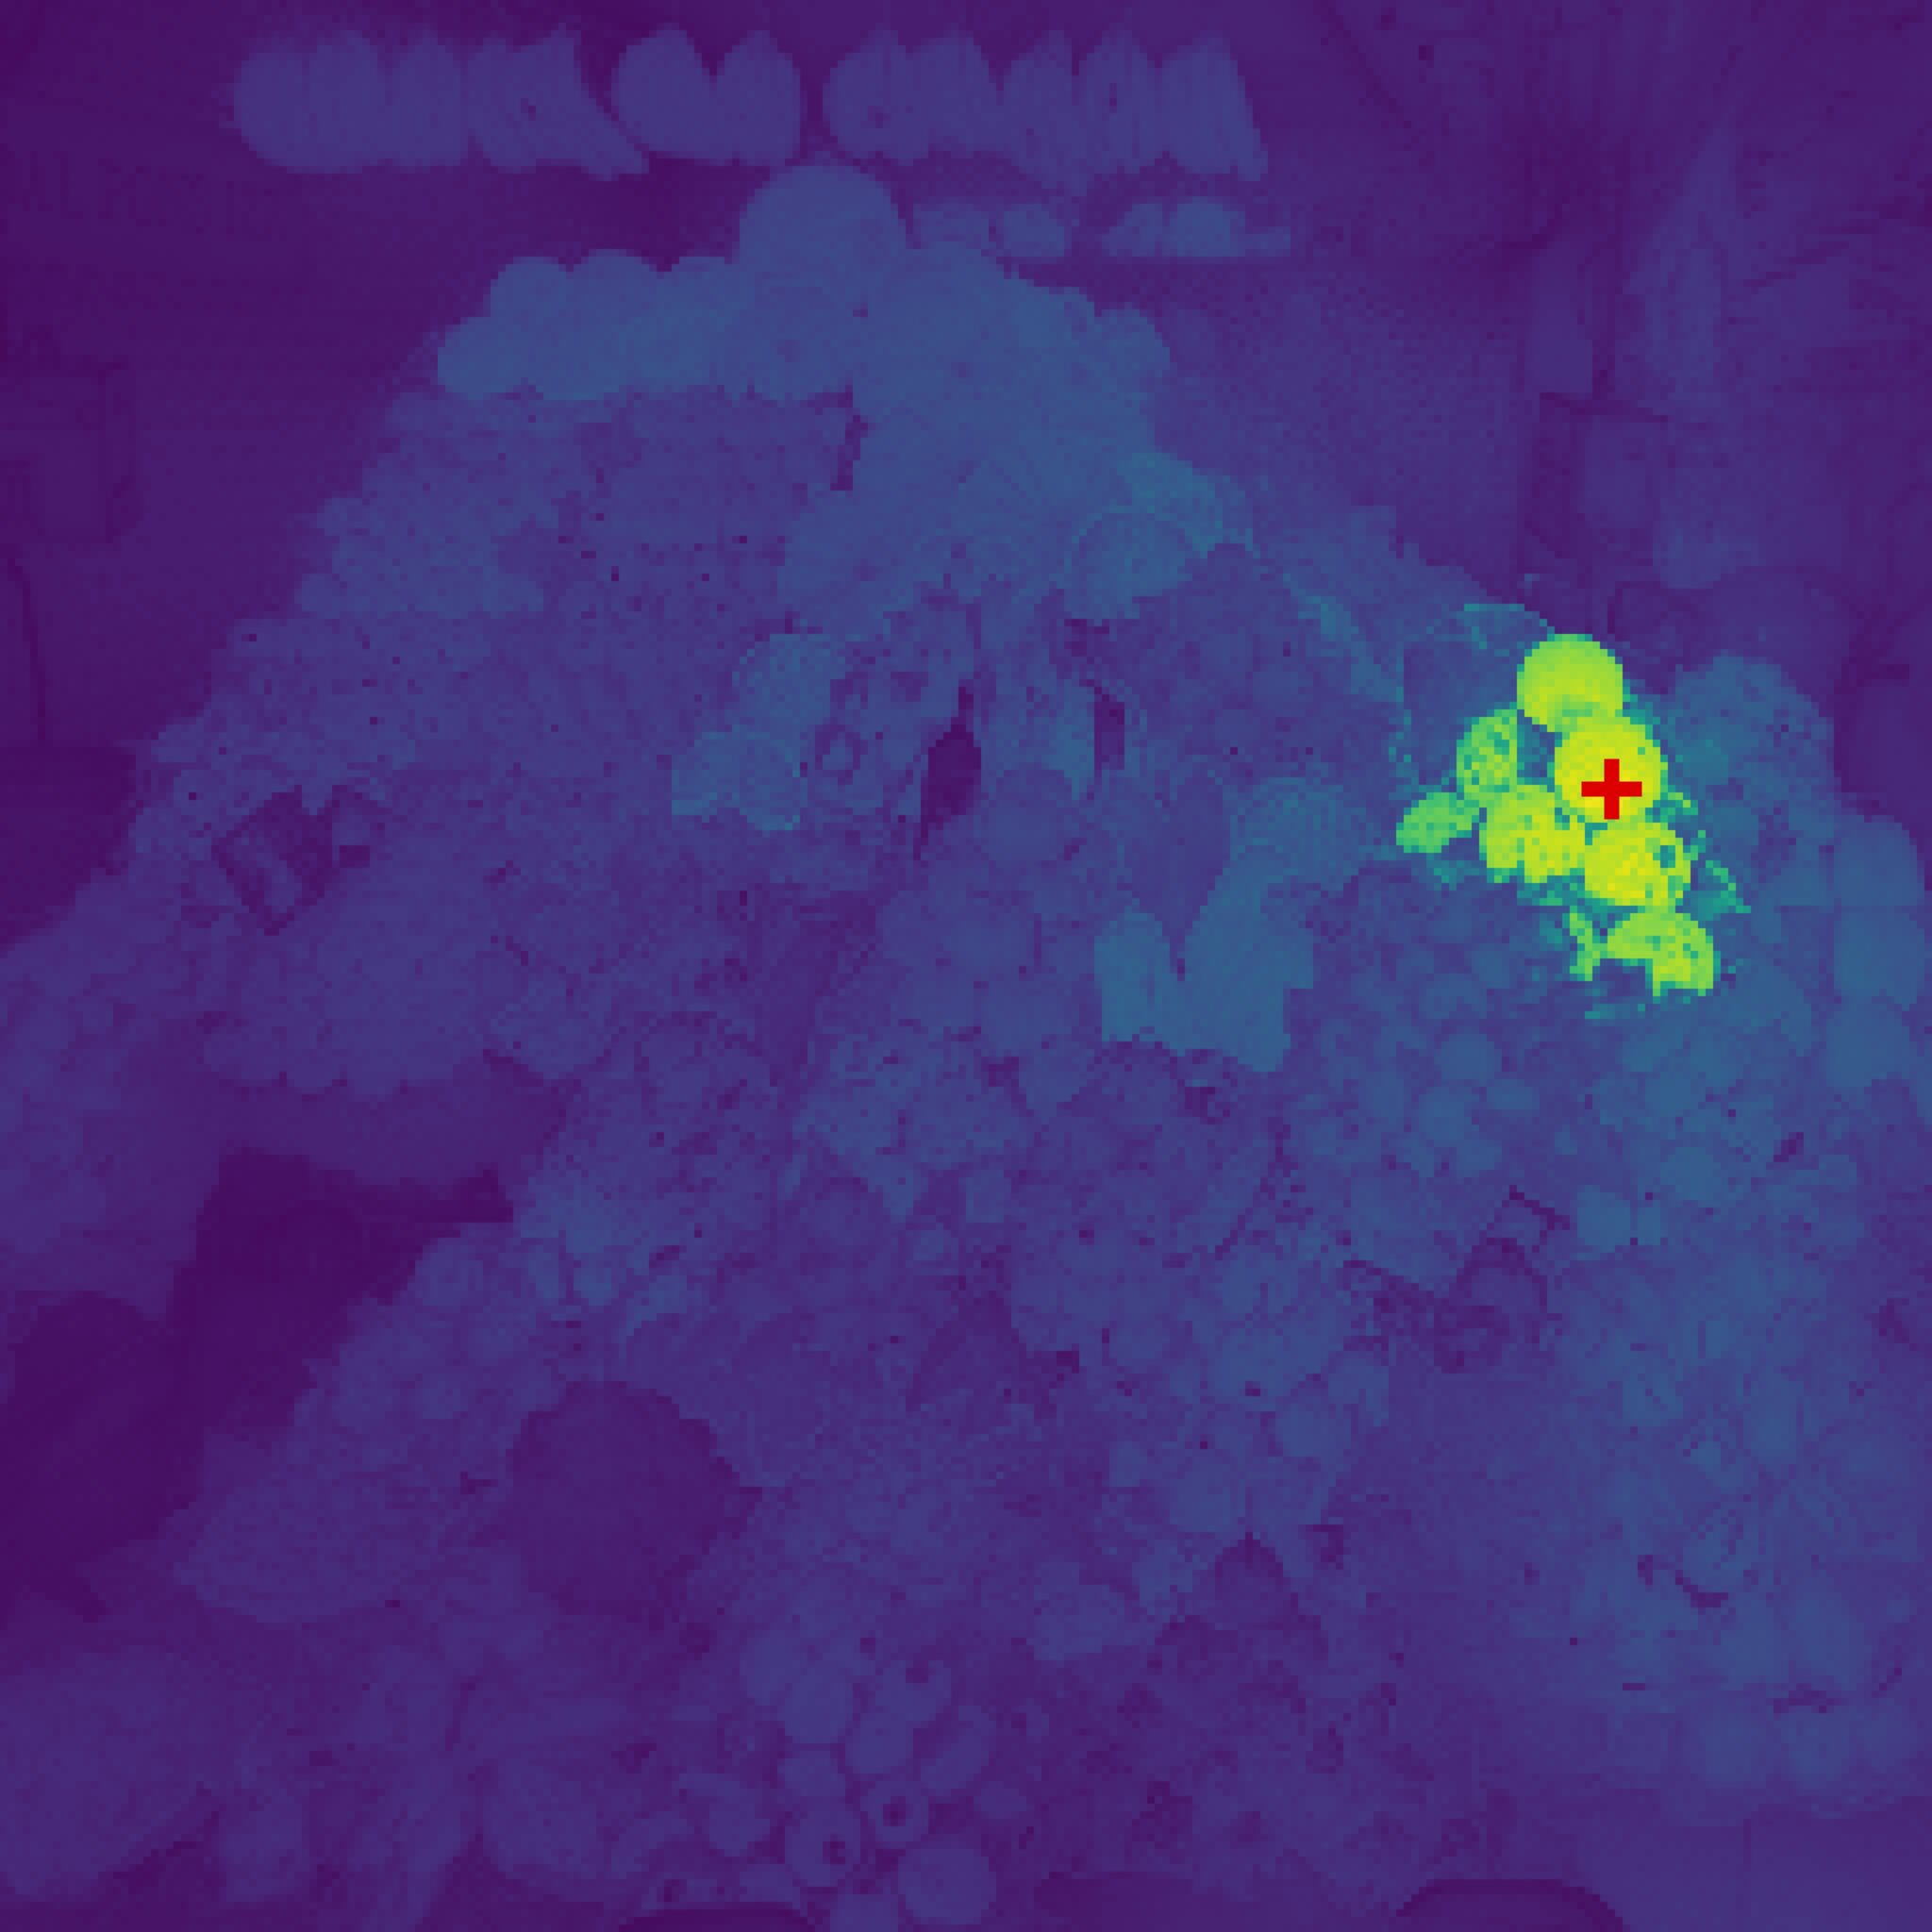
\includegraphics[height=\linewidth, width=\linewidth]{figures/introduction/clutter_scene/viridis_hd/cosmap_1_cross.lr.jpg}\\
    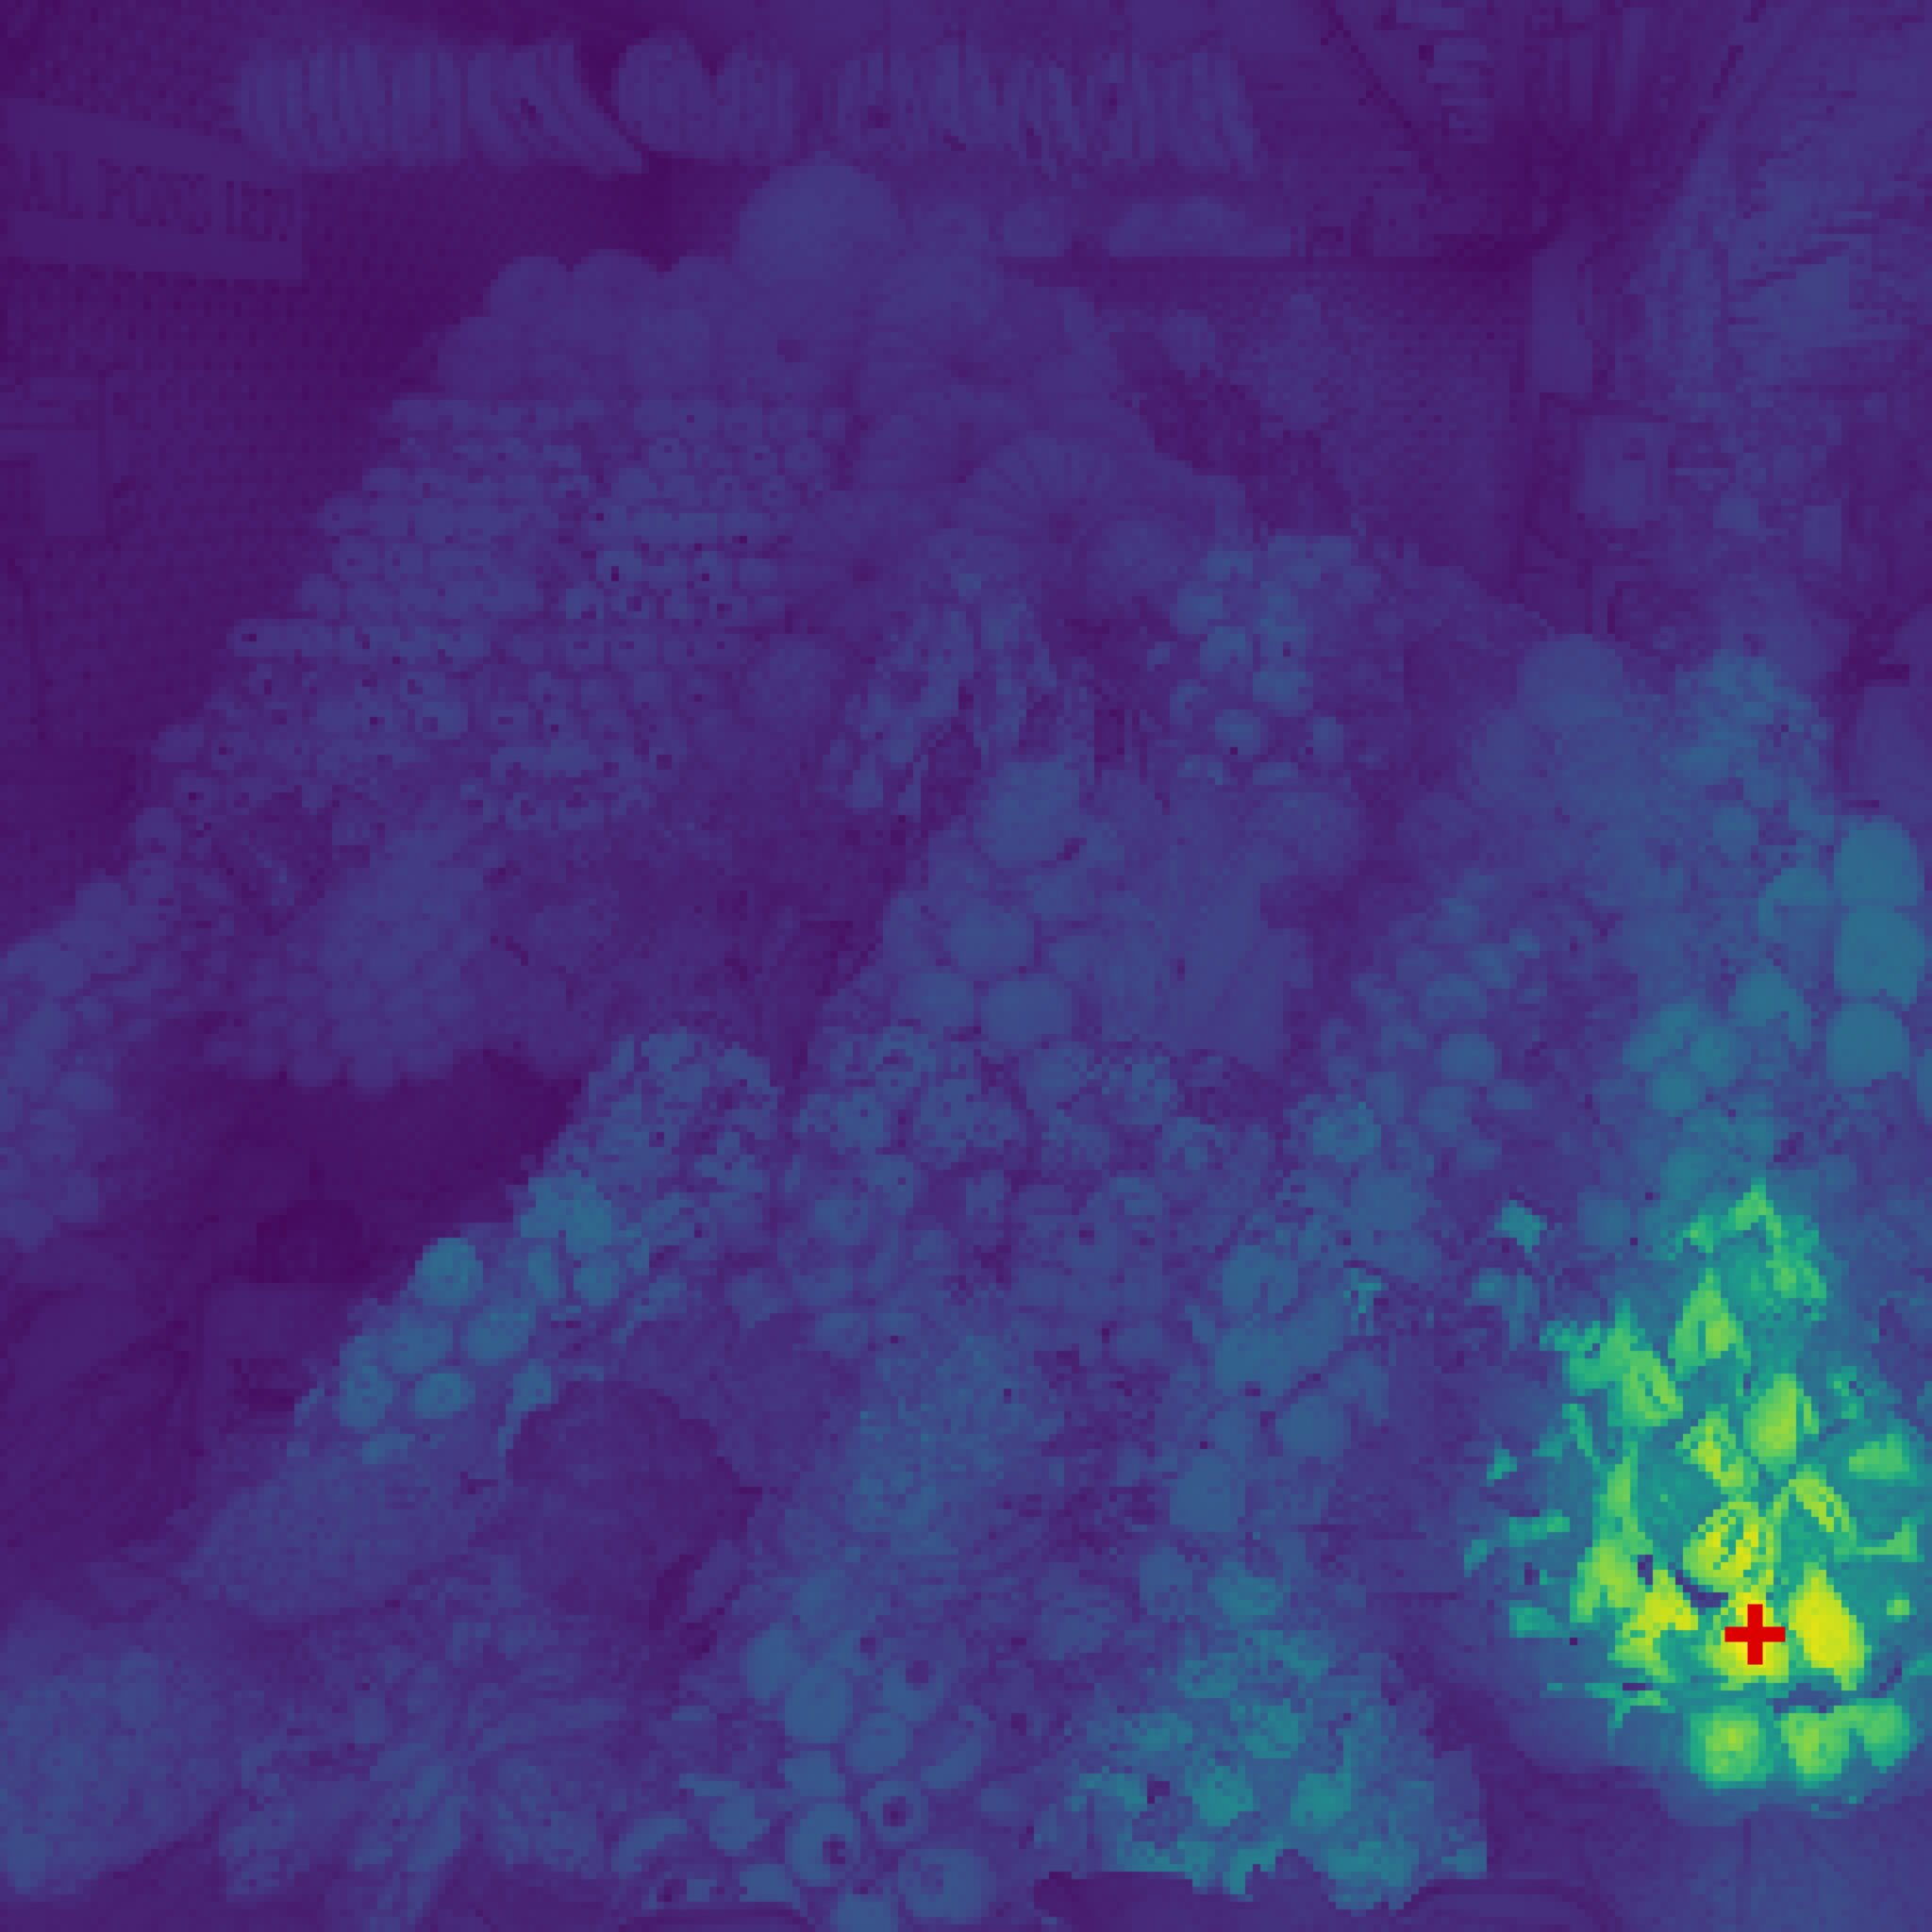
\includegraphics[height=\linewidth, width=\linewidth]{figures/introduction/clutter_scene/viridis_hd/cosmap_5_cross.lr.jpg}
\end{minipage}     
\caption{High-resolution dense features. We visualize the cosine similarity maps obtained with DINOv3 output features between the patches marked with a red cross and all other patches. Input image at 4096×4096. \emph{Please zoom in}, do you agree with DINOv3?}
    \label{fig:intro:dense-quality}
\end{figure}

\paragraph{Overview of Contributions}
In this work, we introduce multiple contributions to address the challenge of scaling SSL towards a large frontier model.
We build upon recent advances in automatic data curation~\citep{vo2024automatic} to obtain a large ``background'' training dataset that we carefully mix with a bit of specialized data (ImageNet-1k). 
This allows leveraging large amounts of unconstrained data to improve the model performance. 
This contribution \textbf{(i)} around data scaling will be described in \cref{sec:data}.

We increase our main model size to 7B parameters by defining a custom variant of the ViT architecture.
We include modern position embeddings (axial RoPE) and develop a regularization technique to avoid positional artifacts. 
Departing from the multiple cosine schedules in DINOv2, we train with constant hyperparameter schedules for 1M iterations. 
This allows producing models with stronger performance. 
This contribution \textbf{(ii)} on model architecture and training will be described in \cref{sec:algo}.

With the above techniques, we are able to train a model following the DINOv2 algorithm at scale. 
However, as mentioned previously, scale leads to a degradation of dense features. 
To address this, we propose a core improvement of the pipeline with a \gramname training phase. 
This cleans the noise in the feature maps, leading to impressive similarity maps, and drastically improving the performance on both parametric and non-parametric dense tasks. 
This contribution \textbf{(iii)} on Gram training will be described in \cref{sec:gram}.

Following previous practice, the last steps of our pipeline consist of a high-resolution post-training phase and distillation into a series of high-performance models of various sizes.
For the latter, we develop a novel and efficient single-teacher multiple-students distillation procedure. 
This contribution \textbf{(iv)} transfers the power of our 7B frontier model to a family of smaller practical models for common usage, that we describe in \cref{sec:distillation}.

As measured in our thorough benchmarking, results in \cref{sec:results} show that our approach defines a new standard in dense tasks and performs comparably to CLIP derivatives on global tasks. 
In particular, \textit{with a frozen vision backbone}, we achieve state-of-the-art performance on longstanding computer vision problems such as object detection (COCO detection, mAP 66.1) and image segmentation (ADE20k, mIoU 63.0), outperforming specialized fine-tuned pipelines. 
Moreover, we provide evidence of the generality of our approach across domains by applying the DINOv3 algorithm to satellite imagery, in \cref{sec:satellite}, surpassing all prior approaches. 
